\documentclass[sigconf,anonymous]{acmart}

%% CBSoft uses an ACM-like format without the ACM Reference block.
%% The following warning from acmart can be safely ignored:
%% "ACM reference format is mandatory for papers over one page."
\settopmatter{printacmref=false}
\renewcommand\footnotetextcopyrightpermission[1]{} % removes footnote with conference information in first column

%% CBSoft uses an ACM-like format without a copyright note.
\setcopyright{none}

%% SBES 2026 conference metadata
\acmConference[SBES 2026]{40th Brazilian Symposium on Software Engineering}{September 8--12, 2026}{São Paulo, SP, Brazil}

%% BibTeX command
\AtBeginDocument{
    \providecommand\BibTeX{{Bib\TeX}}
}

%% Paper written in ENGLISH — keep default Abstract/Keywords/References labels
%% If switching to Portuguese, uncomment the following three lines:
%\renewcommand\abstractname{Resumo}
%\renewcommand\keywordsname{Palavras-chave}
%\renewcommand\refname{Referências}

%% Additional packages
\usepackage{booktabs}   % For high-quality tables
\usepackage{multirow}   % For multi-row table cells
\usepackage{xcolor}     % For colored text (e.g., TODO markers)
\usepackage{listings}   % For code listings if needed
\usepackage{graphicx}   % For including figures
\usepackage{mdframed}   % For finding boxes

%% Path to figures (relative to the paper/ compilation directory)
\graphicspath{{../analysis/figures/}{../results/rq2/}{../results/rq3/}}

%% Finding-box environment
\newmdenv[
  linecolor=black!55,
  linewidth=0.75pt,
  backgroundcolor=black!4,
  innertopmargin=5pt,
  innerbottommargin=5pt,
  innerleftmargin=7pt,
  innerrightmargin=7pt,
  skipabove=8pt,
  skipbelow=4pt,
]{findingbox}

%% TODO command for draft annotations (remove before submission)
\newcommand{\TODO}[1]{\textcolor{red}{\textbf{[TODO: #1]}}}

% ============================================================
\begin{document}

%% Title
\title{How Do AI Agents Resolve Merge Conflicts? An Empirical Study of Conflict Resolution Strategies in AI-Authored Pull Requests}

%% Authors (hidden during double-anonymous review)
\author{FirstName Surname}
\affiliation{
  \institution{Department, University}
  \city{City}
  \country{Country}
}
\email{email@email.com}

\author{FirstName Surname}
\affiliation{
  \institution{Department, University}
  \city{City}
  \country{Country}
}
\email{email@email.com}

%% Short author list for page headers
\renewcommand{\shortauthors}{Surname et al.}
\renewcommand{\shorttitle}{How Do AI Agents Resolve Merge Conflicts?}

% ============================================================
% Abstract
% ============================================================
\begin{abstract}
AI-powered coding agents (Claude Code, OpenAI Codex, GitHub Copilot, Cursor, and Devin) now contribute at scale to open-source repositories through pull requests. When these branches incorporate upstream changes via merge commits, textual conflicts arise and must be resolved by the agent or a human. We present a large-scale empirical study of merge conflicts in AI-authored PRs, covering approximately 930{,}000 PRs across 116{,}000 repositories from the AIDev catalogue. For each PR we identify internal merge commits, reproduce them with \texttt{diff3}, localize each resolution, and classify it into one of seven strategies following \citet{ghiotto2020nature}. Our pipeline recovers $40{,}017$ distinct merges across $210{,}902$ PRs in $57{,}582$ repositories; $25.6\%$ produce at least one conflict, yielding $98{,}322$ chunks. Among classifiable chunks, $74.4\%$ adopt one side verbatim (V1~$50.5\%$, V2~$23.9\%$), matching the $75\%$ reported for human Java merges; agents introduce new code less often ($10.4\%$ vs.\ $13\%$). Conflict incidence varies more than $6{\times}$ across agents, from Copilot ($7.8\%$) to Cursor ($46.1\%$), and most conflicting merges are structurally small (median~2 chunks). The resolver is the agent itself in just $5.8\%$ of merges, ranging from $0.6\%$ (Copilot) to $19.3\%$ (Devin), and a human in $94.1\%$. When agents resolve autonomously, they select~V1 in $86.6\%$ of chunks versus $45.2\%$ for humans (Cram\'{e}r's~$V{=}0.28$, moderate effect), with almost no new-code resolutions ($3.2\%$ vs.\ $11.5\%$). These findings establish the first empirical baseline for merge-conflict behavior in agentic AI and reveal a sharp divide between human and agent resolution strategies.
\end{abstract}

%% Keywords
\keywords{Merge Conflicts, AI Agents, Conflict Resolution, Software Merging, Empirical Software Engineering}

\frenchspacing
\maketitle

% ============================================================
% 1. Introduction
% ============================================================
\section{Introduction}
\label{sec:introduction}

The increasing adoption of AI-powered coding agents, such as Claude Code, OpenAI Codex, GitHub Copilot, Cursor, and Devin, represents a paradigm shift in software development workflows. These agents autonomously create branches, implement features, and open pull requests (PRs) in open-source repositories, contributing code alongside human developers.

When an AI-authored branch needs to incorporate upstream changes (e.g., via \texttt{git merge main}), textual merge conflicts may arise. These conflicts must be resolved before the merged code can be committed, and the resolution may be performed by the AI agent itself, by a human developer, or collaboratively.

Despite the growing scale of AI contributions (the AIDev catalogue~\cite{liaidev2026} alone documents over 930{,}000 AI-authored PRs across 116{,}000 repositories), the nature of the merge conflicts produced inside these PRs remains largely unexplored. Prior work on merge conflict resolution has focused exclusively on human developers~\cite{ghiotto2020nature,vale2022challenges,dinella2022deepmerge,svyatkovskiy2022mergebert,dong2023mergegen}, leaving fundamental questions unanswered in the agentic AI context.

In this paper, we conduct a large-scale empirical study to characterize the nature of merge conflicts that occur inside AI-authored pull requests. Our main contributions are: (i)~the first characterization of the structural nature of merge conflicts in AI-authored branches at scale; (ii)~a comparison of resolution strategies against the human baseline of \citet{ghiotto2020nature}; (iii)~an analysis of who resolves these conflicts and how the strategy profile differs by resolver; and (iv)~an open replication package containing all collection and analysis scripts. Specifically, we address the following research questions:

\begin{itemize}
    \item \textbf{RQ1: Structural nature.} In merge commits that occur inside agent-authored PRs, what are the distributions of (i)~the number of conflicting chunks per failed merge, (ii)~the size in lines of code of each side of the conflict (\emph{v1}, \emph{v2}), and (iii)~the size in lines of code of the resolution?
    \item \textbf{RQ2: Resolution strategies.} How are resolution decisions distributed across conflicting chunks (V1, V2, CC, CB, NC, NN), and how does this distribution compare to the one reported by \citet{ghiotto2020nature} for human-authored merges?
    \item \textbf{RQ3: Resolver.} Who resolves these conflicts: the coding agent itself or a human collaborator?
\end{itemize}

Section~\ref{sec:background} presents background and related work. Section~\ref{sec:methodology} describes our methodology and pipeline. Section~\ref{sec:results} reports results for each RQ. Section~\ref{sec:discussion} discusses implications. Section~\ref{sec:threats} addresses threats to validity, and Section~\ref{sec:conclusion} concludes.

% ============================================================
% 2. Background and Related Work
% ============================================================
\section{Background and Related Work}
\label{sec:background}

\subsection{Software Merging and Merge Conflicts}
\label{sec:bg-merging}

Collaborative software development relies on branching, whereby developers work in parallel on independent copies of a code base and later reconcile their contributions via \emph{merging}~\cite{mens2002survey}. Unstructured three-way merge, as implemented by \texttt{git merge}, compares each pair of versions against their common ancestor and automatically combines non-overlapping edits~\cite{mens2002survey,ghiotto2020nature,cavalcanti2019}. When both sides edit the same textual region, the merger reports a \emph{conflict} and delegates resolution to the developer. Git records conflicting regions with the familiar \verb|<<<<<<<|, \verb|=======|, and \verb|>>>>>>>| markers, and the \texttt{diff3} output additionally preserves the common ancestor between \verb+|||||||+ and \verb|=======|, yielding the three-way view on which subsequent analyses depend~\cite{ghiotto2020nature,dinella2022deepmerge}.

Merge conflicts are frequent and costly. \citet{ghiotto2020nature} inspected 960{,}366 merge scenarios across 2{,}731 open-source Java projects and found that 11.9\% produced at least one conflict, yielding 175{,}805 conflicting chunks. Similar rates (10--20\%) have been reported across ecosystems~\cite{ghiotto2020nature,vale2022challenges,lessenich2018indicators}. \citet{vale2022challenges} combined the mining of roughly 81{,}000 merge scenarios from 66 projects with a developer survey and identified four recurring challenges: understanding the conflict, making the correct resolution decision, dealing with tooling, and coordinating with teammates. \citet{lessenich2018indicators} combined a developer survey with a mining study of 163 projects and showed that the indicators developers \emph{believe} predict conflicts correlate only weakly with measured conflict rates, motivating data-driven investigations. \citet{nelson2019lifecycle} complemented these quantitative findings with a qualitative life-cycle study, documenting the understand--plan--resolve--verify workflow and the heuristics developers employ (e.g., prefer the newer change, prefer the one they authored). Resolution time correlates with the number, size, and structural complexity of conflicting chunks, as well as with the familiarity of the developer with the affected code.

Several lines of work look beyond line-based merging. \citet{apel2011semistructured} introduced \emph{semistructured merge}, which parses artifacts only up to a user-chosen granularity (e.g., declaration boundaries) and thereby avoids many spurious textual conflicts without requiring a full syntactic analysis. Building on this foundation, \citet{cavalcanti2019} compared unstructured, semistructured, and fully structured merge over 40{,}000+ scenarios and showed that language-aware merging eliminates a substantial portion of \emph{false-positive} conflicts (edits that are syntactically independent) while introducing a smaller number of \emph{false-negative} semantic conflicts. \citet{accioly2018semistructured} further characterized the specific classes of Java conflicts that semistructured merge resolves and those that remain. A complementary line targets conflict \emph{avoidance} rather than resolution: \citet{brun2011proactive} introduced \textsc{Crystal}, which speculatively merges branches in the background and surfaces conflicts before the developer attempts the merge, and \citet{kasi2013cassandra} reorder pending tasks so that conflicts are less likely to materialize in the first place. Finally, \citet{boll2024semi} revisited the assumption that conflicts require human judgment: analyzing 131{,}154 resolutions, they found that 87.9\% of conflicting chunks could be derived by a small, language-agnostic catalogue of resolution patterns, suggesting that semi-automation is more feasible than previously assumed. These studies collectively motivate systematic, data-driven investigations of how conflicts are actually resolved, the gap this paper addresses for AI-authored pull requests.

\subsection{Merge Conflict Resolution Strategies}
\label{sec:bg-strategies}

\paragraph{Taxonomy of resolutions.}
\citet{ghiotto2020nature} introduced the canonical taxonomy that classifies each resolved chunk by comparing the merged text against the two conflicting versions ($v_1$, $v_2$): the developer may adopt one version verbatim (\textit{V1}, \textit{V2}), concatenate both sides in either order (\textit{ConcatV1V2}, \textit{ConcatV2V1}), interleave tokens or lines from both (\textit{Combination}), write content absent from both sides (\textit{New Code}), or resolve to an empty region (\textit{None}). An additional \textit{Imprecise} label is used when the resolution cannot be reliably mapped to the conflict region (e.g., because the file was substantially reorganized). Across the 175{,}805 Java chunks they studied, \textit{V1} and \textit{V2} together account for 57\% of resolutions, \textit{New Code} for 22\%, and concatenation/combination for 14\%, with \textit{None} (6.7\%) covering trivial or empty resolutions. We adopt this taxonomy, collapsing \textit{ConcatV1V2} and \textit{ConcatV2V1} into a single \textit{CC} label and folding \textit{Combination} into a \textit{CB} class, which gives us six classifiable labels (V1, V2, CC, CB, NC, NN) plus \textit{Imprecise}, directly comparable to the human baseline.

\paragraph{Automated resolution: classification and generation.}
Machine-learning-based resolvers have matured along two paradigms. The \emph{classification} paradigm, pioneered by \textsc{DeepMerge}~\cite{dinella2022deepmerge}, trains pointer-network models to pick a label from a restricted strategy set; on 8{,}719 JavaScript resolutions, \textsc{DeepMerge} classifies 37\% of non-trivial conflicts correctly. \textsc{MergeBERT}~\cite{svyatkovskiy2022mergebert} extends this idea with a Transformer model trained on Java, JavaScript, TypeScript, and C\# data, reaching 63--68\% accuracy on a five-class output space that matches Ghiotto's most frequent strategies. The \emph{generation} paradigm, championed by \textsc{MergeGen}~\cite{dong2023mergegen}, frees the model from a fixed label inventory and synthesizes the resolution text directly; it outperforms \textsc{MergeBERT} on the same benchmarks, confirming that treating merge as a sequence-to-sequence task captures edits (notably \textit{New Code}) that classifiers cannot emit. \textsc{ChatMerge}~\cite{shen2023chatmerge} combines a strategy classifier with ChatGPT to specialize the generation step per class. More recent work has explored search-based alternatives: \textsc{SBCR}~\cite{camposjunior2024sbcr} formulates resolution as a genetic search over candidate lines, achieving 86.5\% median textual similarity to ground-truth resolutions on 9{,}998 chunks, and \citet{camposjunior2022sbes} showed that over 87\% of real-world resolutions can be reconstructed by combining lines already present in the conflicting versions, yielding a 94.7\% reduction in the search space for automated tools. Beyond ML, \citet{pan2021synthesis} applied programming-by-example synthesis to Microsoft Edge/Chromium fork merges and resolved 11.4\% of conflicts automatically using learned templates. \citet{elias2023mestre} proposed \textsc{Mestre}, a data-mining recommender that achieves 80.8\% classification accuracy and auto-resolves 70.5\% of conflicts in 20 projects. \textsc{RPredictor}~\cite{aldndni2023rpredictor} focuses on a simpler three-way decision (keep-local, keep-remote, or manual) and trains per-project classifiers on 74{,}861 conflicts.

\paragraph{Prediction and benchmarks.}
Complementary to resolution, conflict \emph{prediction} aims to warn developers early. \citet{owhadikareshk2019} trained a lightweight classifier on 267{,}657 merge scenarios across seven languages and reported F1 above 0.80 on most projects, without running the full merge. \citet{brindescu2020planning} pushed the prediction target further, using chunk-level features (size, construct, number of edit locations) to estimate the \emph{time} a developer will spend on a conflict, which informs our choice of structural features for RQ1. \textsc{ConflictBench}~\cite{shenmeng2024conflictbench} curates 180 Java scenarios with ground-truth resolutions to standardize the evaluation of merge tools, addressing the reproducibility gap left by project-specific mining studies.

\paragraph{Gap.}
All the studies above treat \emph{humans} as the implicit resolvers. No prior work has characterized the structural nature or the resolution strategies of conflicts in AI-authored branches, nor has any study separated AI-performed from human-performed resolutions in such branches. Our work fills that gap by reusing Ghiotto's structural metrics and strategy taxonomy on a population of merges that only became possible after the recent rise of autonomous coding agents.

\subsection{AI Agents in Software Development}
\label{sec:bg-agents}

The past two years have seen the emergence of autonomous coding agents that go beyond code completion and act as first-class contributors on GitHub. \citet{liaidev2025se3} label this regime \emph{Software Engineering 3.0}, in which agents independently open branches, write code, invoke tests, and submit pull requests that are subsequently reviewed by humans or by other agents. The rise of these agents is anchored in strong quantitative evidence: \citet{peng2023copilot} ran a randomized controlled trial of GitHub Copilot with 95 developers and observed a 55\% speed-up on a realistic programming task, establishing that AI coding assistance materially alters developer workflow. \citet{wang2024llmagents} survey the architectures of LLM-based software-engineering agents (planner, actor, reviewer patterns) and the benchmarks used to evaluate them, most prominently \textsc{SWE-bench}~\cite{jimenez2024swebench}, which requires agents to synthesize a patch that passes the original test suite for a real GitHub issue. Although frontier agents still solve only a minority of \textsc{SWE-bench} instances, the benchmark has become the reference point for measuring progress on real-world coding. The present study targets five representative agents: Anthropic's \textbf{Claude Code}, OpenAI's \textbf{Codex}, GitHub's \textbf{Copilot} (in its agentic mode), \textbf{Cursor} (the Cursor Agent), and Cognition's \textbf{Devin}. Each agent authors commits under a distinctive bot identity (e.g., \texttt{claude[bot]}, \texttt{openai-codex[bot]}, \texttt{copilot[bot]}, \texttt{cursor-agent[bot]}, \texttt{devin-ai-integration[bot]}), which is what makes it possible to attribute branches and resolutions to agents at scale.

Empirical studies of these agents remain scarce. \citet{liaidev2025se3,liaidev2026} characterize \emph{agentic} PRs along dimensions such as acceptance rate, PR size, review turnaround, and topic distribution, using the AIDev dataset (see Section~\ref{sec:bg-agenticflict}). They do not, however, examine how branches are integrated: in particular, whether agents create merge commits, how often those merges conflict, and who resolves the conflicts when they do. \citet{agenticflict2025} make an initial move in that direction by \emph{simulating} a two-way merge between the PR's head and base commits to count conflicts, but their analysis does not examine the actual merge commits on the branch or how those conflicts were resolved. Our work is also informed by earlier studies of bot-authored PRs, most notably \citet{alfadel2023dependabot}, who mined Dependabot security PRs at scale and established the methodology for studying bot contributions on GitHub. Modern coding agents differ from rule-based bots such as Dependabot in that they synthesize open-ended code rather than apply fixed templates, which is precisely why their conflict-resolution behavior warrants a dedicated study. Our study complements this work by analyzing real merge commits within the PR branch, distinguishing AI-driven from human-driven resolutions, and applying the human-centric resolution taxonomy to this new population.

\subsection{The AIDev and AgenticFlict Datasets}
\label{sec:bg-agenticflict}

Two datasets currently underpin empirical research on AI coding agents. \textbf{AIDev}~\cite{liaidev2026} is a large-scale catalogue of agent-authored pull requests mined from the GitHub Archive: it covers 932{,}791 PRs opened by five agents (Claude Code, Codex, Copilot, Cursor, Devin) across 116{,}211 repositories and 72{,}631 developers. AIDev provides the full PR metadata (title, body, diff summary, state, \texttt{base\_oid}, \texttt{head\_oid}, \texttt{merged\_at}) but no conflict information. Throughout this paper we use the two identifiers \texttt{base\_oid} and \texttt{head\_oid} in the sense of the GitHub REST API~\cite{liaidev2026}: given a pull request, \texttt{head\_oid} is the 40-character SHA-1 of the tip commit of the PR's \emph{source} (feature) branch, i.e., the last commit the agent authored, while \texttt{base\_oid} is the SHA-1 of the tip commit of the target branch (typically \texttt{main} or \texttt{master}) at the moment the PR was opened. Together they delimit the range of commits the PR proposes to land. In Git notation, the commits introduced by the PR are exactly \verb|base_oid..head_oid|, and a three-way merge of the PR with its target branch uses \texttt{base\_oid} and \texttt{head\_oid} as the two parent revisions.

\textbf{AgenticFlict}~\cite{agenticflict2025} is built on top of AIDev and adds a first conflict layer: by locally cloning each repository and running a two-way \texttt{git merge} between \texttt{base\_oid} and \texttt{head\_oid}, the authors identify 29{,}609 conflicting PRs among 142{,}652 PRs in 59{,}412 repositories (a 27.67\% simulated-conflict rate), yielding 336{,}380 conflict regions. AgenticFlict's key contribution is demonstrating that conflicts in agent-authored code are frequent and non-trivial; however, the dataset has two limitations that motivate our work. First, the conflicts it reports are \emph{simulated}: they represent the merge conditions at the time of PR closure (for closed but unmerged PRs) or data collection (for open PRs), but they do not correspond to any real merge commit performed in the wild. Consequently, the dataset contains no \emph{resolutions}: there is no record of how conflicts were actually handled, because no merge was ever committed. Second, AgenticFlict does not distinguish AI from human actors in the merging process, since no merge actor exists in its simulated setup. Our study addresses both gaps directly from AIDev: we look \emph{inside} each PR branch for real two-parent commits (``internal merges''), reproduce those merges with \texttt{diff3}, localize the accepted resolution for every conflicting chunk in the resulting merge commit, and attribute each resolution to the author of the merge, classifying them as AI or human based on the committer identity.

% ============================================================
% 3. Methodology
% ============================================================
\section{Methodology}
\label{sec:methodology}

Figure~\ref{fig:pipeline} provides an overview of our data collection and analysis pipeline.

\begin{figure}[ht]
 \centering
 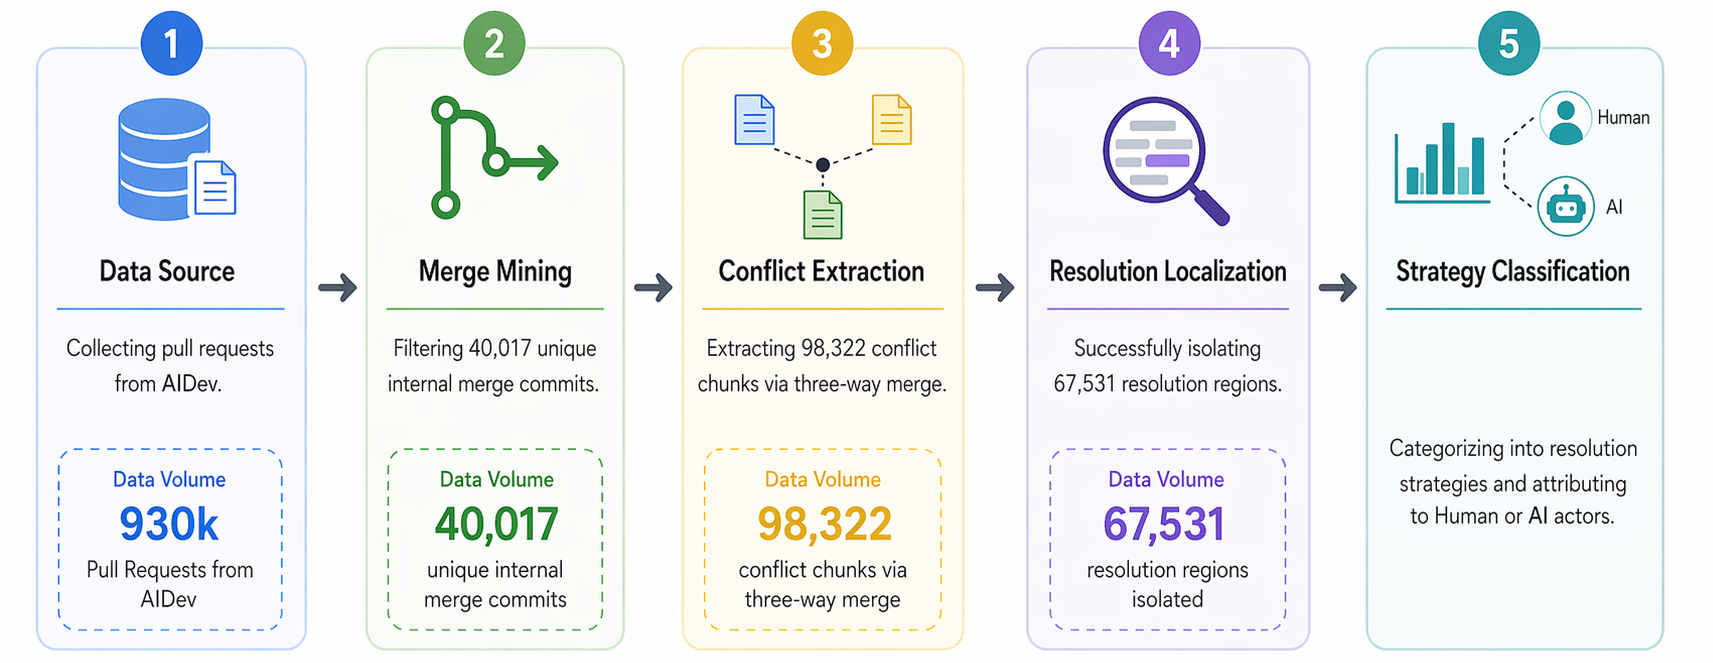
\includegraphics[width=\linewidth]{figures/pipeline}
 \caption{Overview of the data collection and analysis pipeline.}
 \Description{A flowchart showing the five stages of the pipeline: PR selection, merge listing, conflict extraction, authorship collection, and strategy classification.}
 \label{fig:pipeline}
\end{figure}

\subsection{PR Selection and Scope}
\label{sec:meth-selection}

Our study is scoped to the full AIDev catalogue~\cite{liaidev2026}, which documents approximately 930{,}000 pull requests opened by five AI agents (Claude Code, OpenAI Codex, GitHub Copilot, Cursor, and Devin) across roughly 116{,}000 repositories. We consider PRs in all states (\textit{merged}, \textit{closed without merge}, and \textit{open}): restricting to merged PRs would bias the sample toward PRs whose history was rewritten via rebase- or squash-and-merge and would drop exactly the intermediate merge commits we want to study. The per-PR commit inventory needed to locate those internal merges is not shipped with the full AIDev tier; we therefore produce it ourselves by fetching \texttt{refs/pull/*/head} for every in-scope repository and enumerating, per PR, the commits between the fork-point with the base branch and the PR tip.

Applying this procedure to the full AIDev catalogue yields an in-scope dataset of $210{,}902$ pull requests across $57{,}582$ distinct repositories. Our commit-chronology extractor (Pass A) could not produce a complete SHA list for $25{,}571$ of these PRs ($12.1\%$): $20{,}439$ had no resolvable common ancestor between the PR tip and the base branch (\texttt{no\_merge\_base}), typically because the repository history had been force-pushed or heavily rebased after the PR was created; $5{,}132$ had their PR head reference (\texttt{refs/pull/*/head}) no longer accessible at cloning time (\texttt{pr\_ref\_not\_found}); and $735$ raised general exceptions. These PRs contribute no commit data and therefore no internal merge commits to our analysis. Table~\ref{tab:scope-per-agent} reports the per-agent distribution: as in AIDev itself, OpenAI Codex dominates the dataset (approximately 76\% of in-scope PRs), with GitHub Copilot, Cursor, Devin, and Claude Code covering the long tail.

\subsection{Identifying Merge Commits Within PR Branches}
\label{sec:meth-merges}

For each PR, we identify merge commits (commits with exactly two parents) from the set of SHAs produced by the chronology step. These are merges that the PR author (or collaborators) created to bring upstream changes into the feature branch, typically via \texttt{git merge main}, and they are distinct from the single ``integration merge'' that GitHub creates when a PR is accepted. We exclude octopus merges (three or more parents), following \citet{ghiotto2020nature}, and the GitHub integration merge itself: any two-parent commit whose subject matches \texttt{\textasciicircum{}Merge pull request \#$d$+} (case-insensitive) is filtered out, because GitHub's own pre-merge check gates the PR and makes those merges almost always conflict-free. Across the full in-scope dataset, this step excluded $59{,}425$ unique integration-merge SHAs (spanning $23{,}582$ PRs) and $54$ octopus-merge SHAs (spanning $5$ PRs).

\paragraph{Merge-level deduplication.} A single physical merge commit can appear on the head branches of several PRs (force-push, re-open, cherry-pick), so a naive \texttt{(pr\_id, merge\_sha)} indexing overcounts the same physical artefact. All merge- and chunk-level statistics in this paper are therefore computed on natural keys that ignore \texttt{pr\_id}: \texttt{(repo\_full\_name, merge\_sha)} for merges and \texttt{(repo\_full\_name, merge\_sha, file\_path, chunk\_index)} for chunks.

Applying these filters to the in-scope dataset returns $299{,}098$ raw \texttt{(pr\_id, merge\_sha)} pairs, which collapse to $40{,}017$ distinct physical merge commits after deduplication on \texttt{(repo\_full\_name, merge\_sha)}, an inflation factor of $7.47\times$ between the raw PR-level indexing and the true physical artefact. In fact, $62.1\%$ of physical merge commits are referenced by two or more PRs, and the most extreme case is a single merge that appears on the head branches of $727$ distinct PRs. A total of $19{,}214$ PRs ($9.1\%$ of the in-scope dataset) contribute at least one internal merge; the remaining $91\%$ land as fast-forwards, as squash-merges, or are closed without merging, and therefore do not expose a merge commit inside the PR's branch history.

\subsection{Reproducing Merges and Extracting Conflict Chunks}
\label{sec:meth-conflicts}

For each merge commit with parents $p_1$ and $p_2$, we compute the merge base ($b = \text{merge-base}(p_1, p_2)$) and identify files modified on both sides using \texttt{git merge-tree}. For each such file, we reproduce the three-way merge using:

\begin{verbatim}
git merge-file -p --diff3 p1_file base_file p2_file
\end{verbatim}

We parse the resulting diff3 output to extract individual conflict chunks, each delimited by \texttt{<<<<<<<}, \texttt{|||||||}, \texttt{=======}, and \texttt{>>>>>>>} markers. Each chunk produces three text regions: \textit{v1} (from $p_1$), \textit{base} (from $b$), and \textit{v2} (from $p_2$).

\subsection{Localizing the Resolution}
\label{sec:meth-resolution}

For each conflict chunk, we retrieve the resolved file from the merge commit itself via \texttt{git show \{merge\_sha\}:\{file\_path\}}. Since this file contains the entire contents, including non-conflicting regions and other resolutions, we must isolate the specific resolution text corresponding to each chunk. We adopt the \textsc{LocalizeResRegion} algorithm introduced by \citet{dinella2022deepmerge}, which uses contextual anchoring to identify resolution boundaries.

The algorithm works by identifying the prefix and suffix surrounding the conflict region in the three-way merge output and locating their unique occurrences in the resolved file. Specifically, it finds the minimal non-empty prefix (working forward from the conflict) and the minimal non-empty suffix (working backward) that appear uniquely in the resolved file to ``bookend'' the resolution. To ensure robustness, the method prepends a start-of-file token ($\langle BOF \rangle$) and appends an end-of-file token ($\langle EOF \rangle$) to the prefix and suffix, respectively. If the bookends cannot be uniquely identified, the resolution is marked as \textit{Imprecise}.

\citet{dinella2022deepmerge} validated \textsc{LocalizeResRegion} by manually inspecting 174 conflict regions from 50 randomly selected merges, finding that the algorithm correctly localized the resolution in all 174 cases (yielding a 95\% confidence interval of $[0.979, 1.0]$ for accuracy). Given this high reported performance, we use the algorithm confidently to extract resolution regions in our study.

A more subtle threat arises from the \emph{differential Imprecise rate} between resolver types: agent-resolved chunks fail to localize in only $13.4\%$ of cases, versus $40.8\%$ for human-resolved chunks. Because $V_1$ resolutions are structurally simpler (the resolution text precisely matches one parent), they are also easier for the localization algorithm to anchor. The agent's high $V_1$ rate and its low Imprecise rate may therefore be mutually reinforcing: the agent's preference for simple resolutions makes localization easier, which in turn makes agent chunks more likely to appear in the classifiable fraction as $V_1$. We cannot fully disentangle the two effects; readers should interpret the resolver-conditional strategy distribution in Section~\ref{sec:rq3} with this caveat in mind. An upper-bound sensitivity analysis (treating all Imprecise chunks as $V_1$) and a lower-bound analysis (treating them as NC) are provided in the supplementary material.

\subsection{Classifying Resolution Strategies}
\label{sec:meth-strategies}

We classify each resolved chunk into one of seven resolution strategies, following the taxonomy consolidated by \citet{ghiotto2020nature}. The \texttt{identify\_resolution} function compares the normalized resolution text against \textit{v1} and \textit{v2} and emits one of:

\begin{itemize}
    \item \textbf{V1} / \textbf{V2}: The resolution is identical to one side of the conflict.
    \item \textbf{CC} (\emph{Concatenation}): The resolution is the concatenation of both sides, in either order (internally the function distinguishes \texttt{ConcatV1V2} and \texttt{ConcatV2V1}; we fold both into \textit{CC} to stay comparable with \citet{ghiotto2020nature}).
    \item \textbf{CB} (\emph{Combination}): The resolution interleaves lines from \textit{v1} and \textit{v2} without introducing new lines.
    \item \textbf{NC} (\emph{New Code}): The resolution introduces content not present in either side.
    \item \textbf{NN} (\emph{None}): The resolution is empty.
    \item \textbf{Imprecise}: The resolution could not be reliably isolated by the localization algorithm (Section~\ref{sec:meth-resolution}) and is reported as its own bucket to avoid silent misclassification.
\end{itemize}

\paragraph{Reporting convention for RQ2.} Ghiotto et~al.\ do not have an \textit{Imprecise} bucket. To keep the comparison on the same support, the headline RQ2 distributions in the paper are reported over the six classifiable labels (V1, V2, CC, CB, NC, NN), with the \textit{Imprecise} share reported separately (globally and per stratum) as the fraction of chunks dropped from the classifiable distribution. The audit variant that includes \textit{Imprecise} is produced by the same notebook and is available in the replication package.

\subsection{Identifying the Resolver}
\label{sec:meth-resolver}

We determine who resolved each conflict by analyzing the author and committer metadata of the merge commit. We classify the resolver as \textit{AI}, \textit{Human}, or \textit{Agent-assisted} based on a curated list of known AI agent signatures (e.g., \texttt{claude[bot]}, \texttt{openai-codex[bot]}, \texttt{copilot[bot]}, \texttt{cursor-agent[bot]}, \texttt{devin-ai-integration[bot]}) also used by \citet{liaidev2025se3}.

\subsection{Size Metrics}
\label{sec:meth-size}

For each chunk, we record four size metrics used by RQ1: \texttt{v1\_loc}, \texttt{v2\_loc}, \texttt{base\_loc}, and \texttt{resolution\_loc}. All four are computed as the number of non-blank lines after trimming whitespace (consistent with \citet{ghiotto2020nature}'s \texttt{remove\_empty\_lines} normalization). \texttt{resolution\_loc} is the metric this study adds relative to the characterization of \citet{ghiotto2020nature}.

\subsection{Analyses per Research Question}
\label{sec:meth-analyses}

\textbf{RQ1: Structural nature.} For each of \texttt{\#chunks per merge}, \texttt{v1\_loc}, \texttt{v2\_loc}, and \texttt{resolution\_loc}, we report the distribution (histogram with empirical CDF, median, mean, standard deviation, and the 25/50/75/90/95/99 percentiles) globally and per cross-cutting stratum (agent, language, PR task type). Visualizations follow \citet{ghiotto2020nature} figures to enable direct visual comparison.

\textbf{RQ2: Resolution strategies.} We report the relative frequency of each resolution label (V1, V2, CC, CB, NC, NN) at the chunk level, globally and per stratum, with the \textit{Imprecise} share reported separately (Section~\ref{sec:meth-strategies}). The comparison with \citet{ghiotto2020nature} is numerical and textual (no empirical human dataset is collected in this study).

\textbf{RQ3: Resolver.} We report the distribution of the resolver label (\texttt{agent-resolved}, \texttt{human-resolved}) at the merge-commit level, globally and per stratum.

\paragraph{Statistical analyses.}
All proportions are reported with 95\% Wilson (score) confidence intervals~\cite{wilson1927probable}, which handle small counts better than the normal approximation. For distributional comparisons across agents (RQ1), we use the non-parametric Kruskal-Wallis test followed by post-hoc Dunn tests with Bonferroni correction~\cite{dunn1964multiple}; effect sizes are reported as Cliff's~$\delta$~\cite{cliff1993dominance} since the distributions are heavily right-skewed. For association between categorical variables (RQ2, RQ3), we use chi-squared tests of independence; all chi-squared results are accompanied by the bias-corrected Cram\'{e}r's~$V$~\cite{bergsma2013bias} as the primary effect-size metric ($V{<}0.10$: weak; $0.10$--$0.30$: moderate; ${\geq}0.30$: strong). We report~$V$ rather than~$p$ as the primary summary because at $n{\approx}60{,}000$ chunks virtually any difference yields $p{<}0.001$; magnitude therefore carries more information than statistical significance. A validity caveat applies to all tests: conflict chunks within the same merge commit and across commits within the same repository are not fully independent, so all~$p$-values are anti-conservative (i.e., smaller than they would be under strict independence). All reported~$V$ values are therefore treated as \emph{upper bounds} on the true population effect. Because we do not compare our dataset to \citet{ghiotto2020nature} distribution using a goodness-of-fit test, which is inappropriate given different populations, within-cluster dependence, and power inflation at this sample size; instead, we instead report the absolute percentage-point difference and whether \citet{ghiotto2020nature}'s estimate falls within our 95\% Wilson CI for each strategy.

% ============================================================
% 4. Results
% ============================================================
\section{Results}
\label{sec:results}

\subsection{Dataset Overview}
\label{sec:res-overview}

Our pipeline covers the full AIDev catalogue and recovers, after merge-level deduplication, $40{,}017$ distinct internal merge commits authored inside the $210{,}902$ in-scope PRs across $57{,}582$ repositories (Table~\ref{tab:dataset-overview}). Of those merges, $10{,}232$ ($25.6\%$) produce at least one textual conflict, yielding $98{,}322$ conflict chunks. At the PR level, $19{,}214$ PRs ($9.1\%$) contribute at least one internal merge and $3{,}628$ ($1.7\%$) contain at least one conflicting merge, confirming that internal merges are the exception rather than the rule in agent-authored branches and that conflicts, when they do arise, cluster inside a comparatively small slice of the dataset. The resolution-localization algorithm of \citet{dinella2022deepmerge} uniquely identifies the resolution region for $67{,}531$ of the $98{,}322$ chunks ($68.7\%$); the remaining $31.3\%$ are kept as \emph{Imprecise} and reported separately throughout the paper.

\begin{table}
  \caption{Dataset overview (after merge-level deduplication).}
  \label{tab:dataset-overview}
  \begin{tabular}{lrr}
    \toprule
    Metric & Count & Share \\
    \midrule
    Repositories in scope                 & $57{,}582$  & --- \\
    Pull requests in scope                & $210{,}902$ & --- \\
    PRs with $\geq 1$ internal merge      & $19{,}214$  & $9.1\%$ of PRs \\
    PRs with $\geq 1$ conflicting merge   & $3{,}628$   & $1.7\%$ of PRs \\
    Internal merge commits (dedup.)       & $40{,}017$  & --- \\
    Conflicting merge commits             & $10{,}232$  & $25.6\%$ of merges \\
    Conflict chunks                       & $98{,}322$  & --- \\
    Chunks with localized resolution      & $67{,}531$  & $68.7\%$ of chunks \\
    \bottomrule
  \end{tabular}
\end{table}

\begin{table*}
  \caption{Per-agent scope and conflict incidence.}
  \label{tab:scope-per-agent}
  \begin{tabular}{lrrrr}
    \toprule
    Agent & PRs & Internal merges & Conflicting merges & Conflict rate \\
    \midrule
    OpenAI Codex & $160{,}832$ & $22{,}410$ & $8{,}105$ & $36.2\%$ \\
    Copilot      & $21{,}846$  & $14{,}937$ & $1{,}170$ & $7.8\%$ \\
    Cursor       & $14{,}903$  & $674$      & $311$     & $46.1\%$ \\
    Devin        & $11{,}433$  & $1{,}533$  & $546$     & $35.6\%$ \\
    Claude Code  & $1{,}888$   & $463$      & $100$     & $21.6\%$ \\
    \bottomrule
  \end{tabular}
\end{table*}

\subsection{RQ1: Structural Nature}
\label{sec:rq1}

\paragraph{Chunks per merge.} Across the $10{,}232$ conflicting merge commits, the number of conflicting chunks is heavily right-skewed: the median is $2$, the 75th percentile is $4$, and the 90th percentile is $12$, yet the mean is $9.61$ (standard deviation $108.2$) because the tail reaches $9{,}791$ chunks in a single merge. Three quarters of conflicting merges therefore contain at most four chunks and would be individually tractable, while a long tail of merges, concentrated above the 99th percentile ($122$ chunks), are arbitrarily complex. Restricting the distribution to the $40{,}017$ \emph{all} internal merges, including conflict-free ones, drops the median to $0$ and the 90th percentile to $3$, confirming that most agent-authored internal merges integrate cleanly.

\paragraph{Side sizes.} Chunk-level sizes on the $v_1$ and $v_2$ sides mirror each other closely: the median size is $3$ LOC for $v_1$ and $2$ LOC for $v_2$ after whitespace-only normalization, with 75th percentiles of $14$ and $6$ and 99th percentiles of $280$ and $130$ respectively. The common ancestor (\texttt{base}) is even more compact, with a median of $1$ LOC and a 99th percentile of $98$ LOC, which is consistent with conflicts that arise from tightly-bounded divergent edits. The largest chunk side size is $199{,}765$ ($v_1$) in a conflict in the project \texttt{Bryan-Roe-ai/semantic-kernel}. This outlier case is related to a bulk-refactor generated by Codex on this large mono-repo. 

\paragraph{Resolution size.} The \texttt{resolution\_loc} distribution, the metric this study adds relative to \citet{ghiotto2020nature}, shows a similar skew. The median resolution is $1$ LOC long and the 75th percentile is $6$, closely tracking the median of $v_1$. The tail, however, is heavier: the 99th percentile reaches $1{,}525$ LOC and the maximum $199{,}769$, slightly larger than the largest $v_1$ seen in the sample. This pattern is compatible with a dominant ``pick a side'' behaviour (Section~\ref{sec:rq2}) combined with occasional rewrites that introduce material new content alongside the resolution.

\paragraph{Per-stratum incidence.} Conflict incidence at the PR level varies by agent: Claude Code leads with $3.8\%$ of its $1{,}888$ PRs producing at least one conflict, followed by OpenAI Codex ($1.8\%$ of $160{,}832$), Devin ($1.7\%$ of $11{,}433$), Cursor ($1.2\%$ of $14{,}903$), and Copilot ($1.0\%$ of $21{,}846$). At the merge-commit level the ranking reorders because agents differ in how often they create internal merges at all: Cursor ($46.1\%$ conflict rate among its $674$ internal merges) and OpenAI Codex ($36.2\%$ of $22{,}410$) are the most conflict-prone, whereas Copilot's $14{,}937$ merges yield conflicts in only $7.8\%$ of cases, consistent with Copilot's use of comparatively short-lived feature branches. Python and Java exhibit the highest per-language conflict incidence at the PR level ($2.3\%$ and $1.4\%$ respectively), while Go repositories sit below $1.2\%$.


\begin{figure}[t]
  \centering
  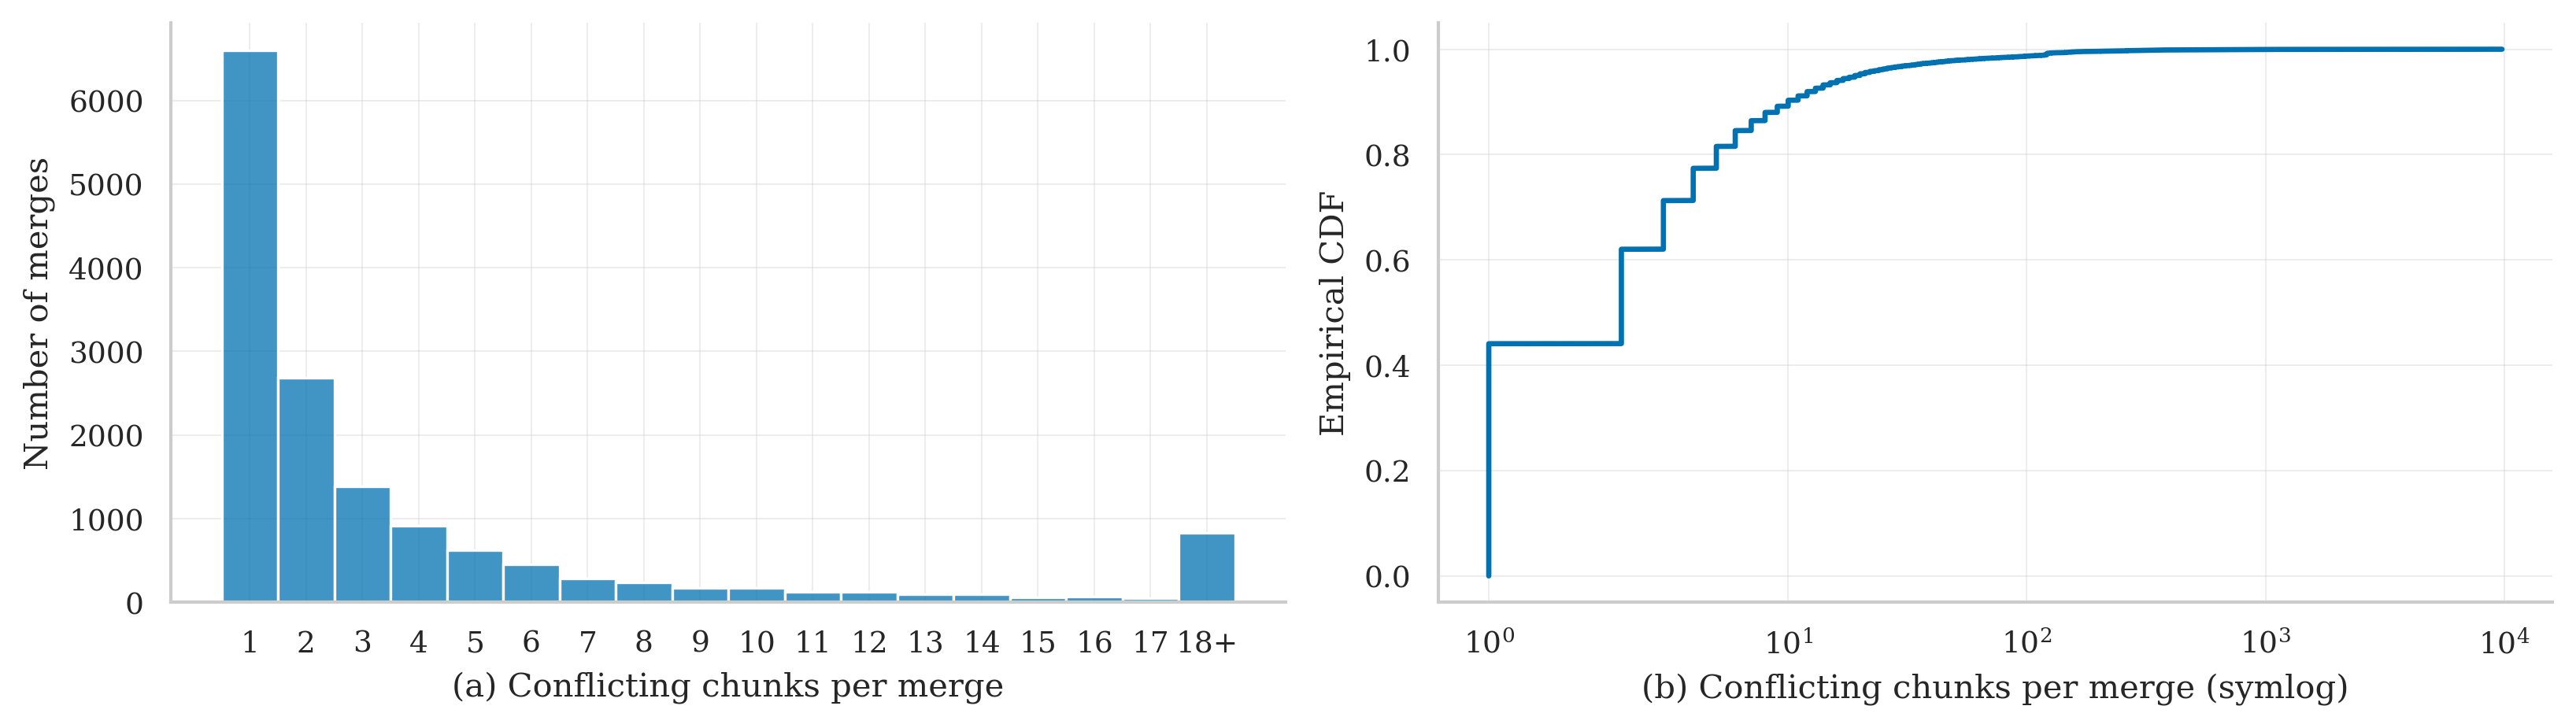
\includegraphics[width=\columnwidth]{rq1_chunks_per_merge_global}
  \caption{Distribution of the number of conflicting chunks per merge commit across all $40{,}017$ internal merges. The median ($2$) and the heavily right-skewed tail are the key structural features of the dataset.}
  \Description{Histogram with an empirical CDF inset, showing most merges have zero or a handful of conflict chunks but a long tail reaches thousands.}
  \label{fig:rq1-chunks-global}
\end{figure}

\begin{figure}[t]
  \centering
  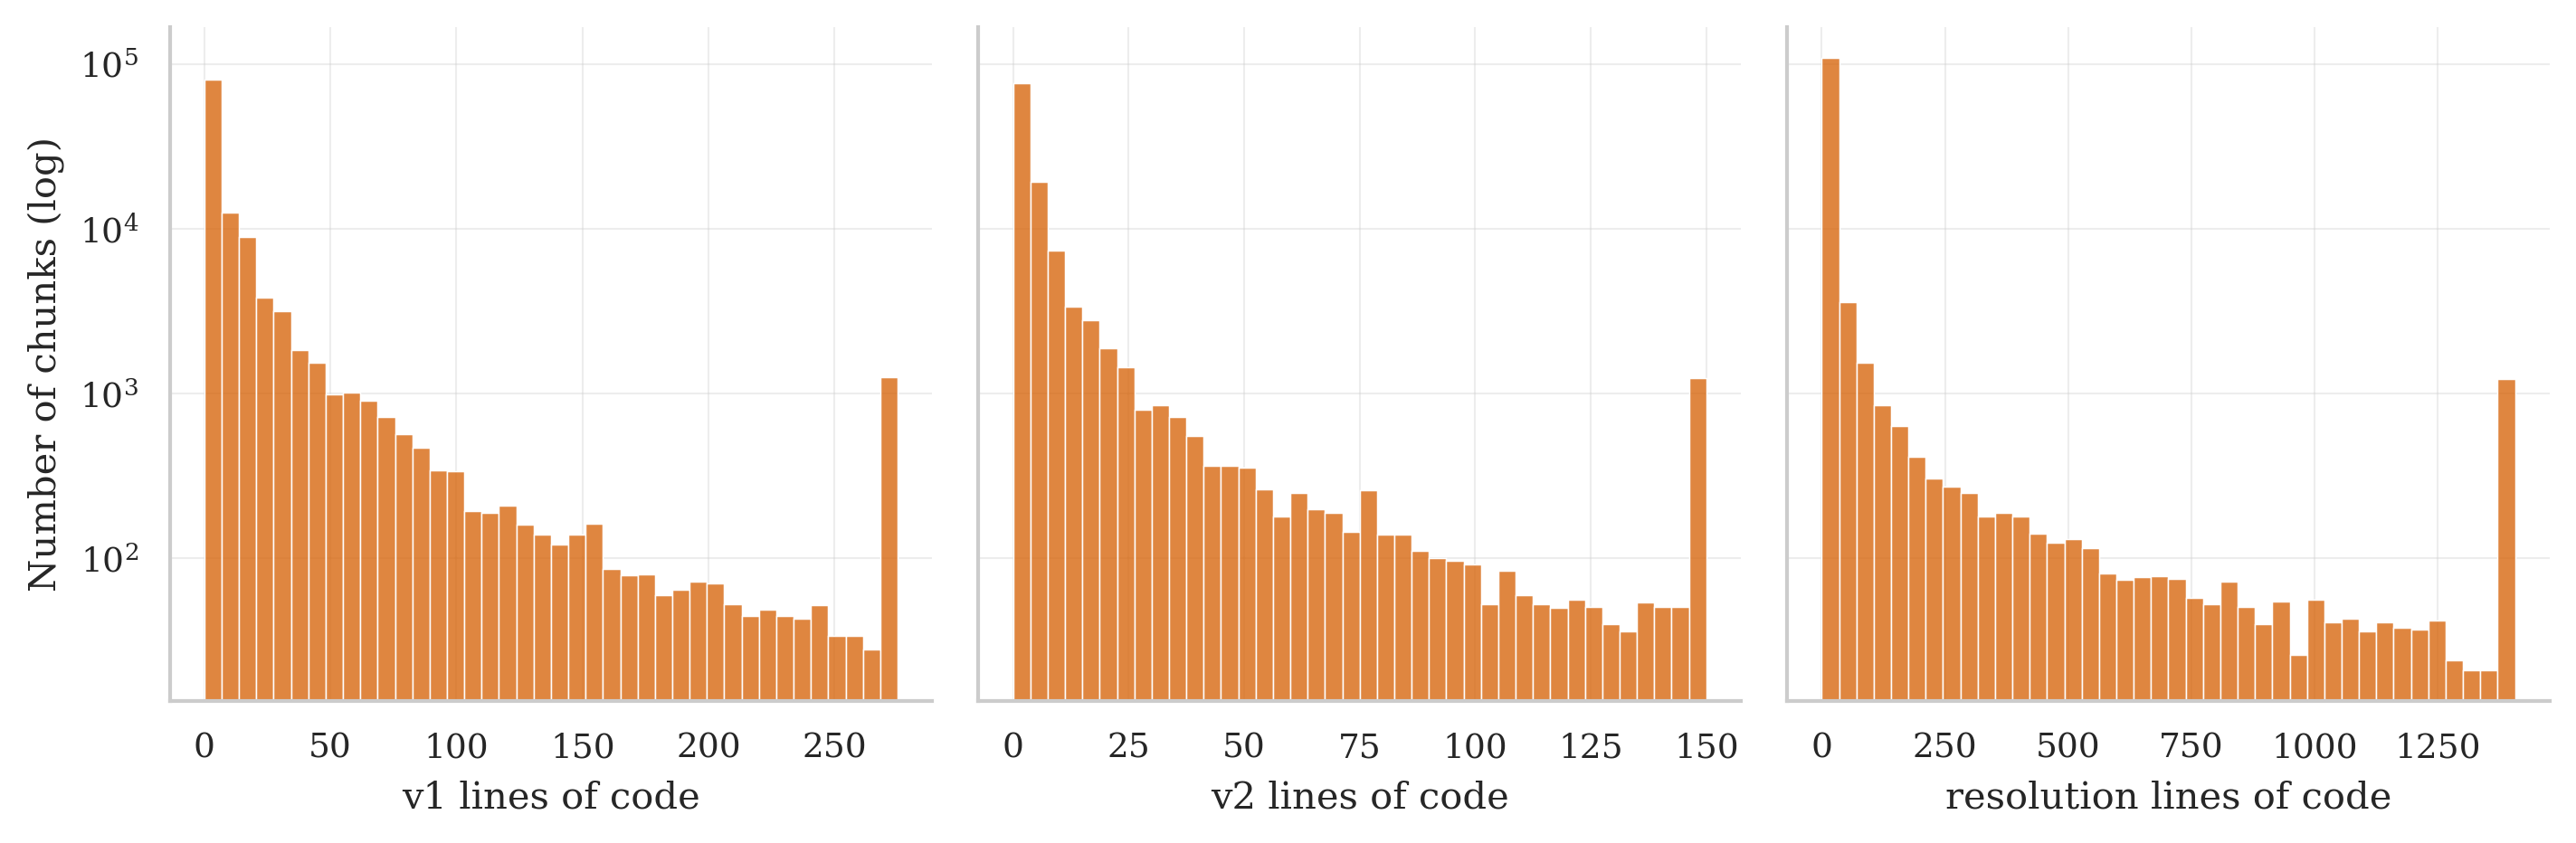
\includegraphics[width=\columnwidth]{rq1_loc_distributions_global}
  \caption{Size distributions (non-blank LOC) of the $v_1$, $v_2$, base, and resolution sides across all $98{,}322$ conflict chunks. All four distributions are heavily right-skewed and concentrated near 1--3~LOC.}
  \Description{Overlapping density or box plots for v1, v2, base, and resolution LOC showing tight concentration near 1-3 lines with heavy right tails.}
  \label{fig:rq1-loc-global}
\end{figure}

\paragraph{Statistical tests.} A Kruskal-Wallis test on the number of conflict chunks per conflicting merge across agents yields $H{=}63.6$ ($p{<}0.001$), indicating that at least one agent differs. Post-hoc Dunn tests (Bonferroni-corrected) reveal that OpenAI Codex differs significantly from both Claude Code ($p{=}0.005$) and Cursor ($p{<}0.001$), while no other pair reaches significance, consistent with Codex's smaller median chunk count ($2$ vs.\ $3$ for Claude Code and Cursor). Effect sizes are uniformly negligible to small (Cliff's~$\delta{<}0.18$ for all pairs), confirming that per-agent differences in the number of chunks per merge, although detectable, are not practically large. LOC distributions (\texttt{v1\_loc}, \texttt{v2\_loc}, \texttt{base\_loc}, \texttt{resolution\_loc}) differ significantly across agents (Kruskal-Wallis $H{=}159$--$2487$, all $p{<}0.001$); interpreting these differences requires controlling for the programming languages targeted by each agent, which differ substantially across the dataset.

\textbf{Summary.} Structurally, merge conflicts in agent-authored branches are \emph{small and common}, with a \emph{long heavy tail}: most conflicting merges contain only a handful of short chunks, but a non-trivial minority (above the 99th percentile) are arbitrarily complex. The median chunk in our population is on the order of one to three lines on each side, and the resolution is of comparable size, placing our observations near the short-chunk end of the \citet{ghiotto2020nature} distribution for human Java merges. Per-agent conflict rates span a full order of magnitude, from Copilot ($7.8\%$, 95\%~CI $[7.4\%,8.3\%]$) to Cursor ($46.1\%$, $[42.4\%,49.9\%]$), underscoring that any tooling informed by conflict prevalence needs to be interpreted against the agent that produced the branch.

\begin{findingbox}
\textbf{Finding 1.} Conflicts in agent-authored merges are structurally small: the median conflicting merge contains~2 chunks, each spanning 2--3 lines per side (Figures~\ref{fig:rq1-chunks-global}--\ref{fig:rq1-loc-global}). The distribution is heavily right-skewed; a small minority of merges above the 99th percentile concentrates most of the conflict workload. \\[3pt]
\textbf{Finding 2.} Conflict incidence at the merge-commit level varies by more than $6\times$ across agents, from~$7.8\%$ (Copilot) to~$46.1\%$ (Cursor), reflecting differences in branching strategy rather than code quality alone.
\end{findingbox}

\subsection{RQ2: Resolution Strategies}
\label{sec:rq2}

\paragraph{Global distribution.} Over the $98{,}322$ conflict chunks, $38.2\%$ are marked \emph{Imprecise} by the localization step and are reported separately (Section~\ref{sec:meth-strategies}); the remaining $60{,}813$ classifiable chunks are the basis of the numbers below and of Figure~\ref{fig:rq2-global-ghiotto}. Among classifiable chunks, \textbf{$74.4\%$ of resolutions take one side verbatim} ($V_1$ $50.5\%$, $V_2$ $23.9\%$), $14.6\%$ mix the two sides (\emph{CC} $5.5\%$, \emph{CB} $9.1\%$), $10.4\%$ introduce new code not present in either parent (\emph{NC}), and $0.6\%$ resolve to an empty region (\emph{NN}). For direct comparison, \citet{ghiotto2020nature} report that humans resolving Java conflicts pick a single side in $75\%$ of chunks, mix sides in $12\%$, and write new code in $13\%$. Agents are therefore \emph{comparable to humans in picking one side verbatim} ($74.4\%$ vs.\ $75\%$), \emph{slightly less likely to introduce new code} ($10.4\%$ vs.\ $13\%$), and \emph{slightly more likely to mix} ($14.6\%$ vs.\ $12\%$). Taken together, agent-authored conflicts are resolved with a \textbf{conservative playbook}.

\paragraph{Per-agent breakdown.} The $V_1$ bias is strongest in Copilot (excl.\ Imprecise: $V_1$ $59.2\%$, $V_2$ $20.0\%$) and OpenAI Codex ($V_1$ $50.8\%$, $V_2$ $23.0\%$), both of which drive the global distribution by volume. Claude Code and Devin invert the polarity, favouring $V_2$ ($43.3\%$ and $42.3\%$ respectively against $V_1$ at $33.1\%$ and $31.0\%$); Cursor sits in between ($V_1$ $40.3\%$, $V_2$ $25.6\%$). The \emph{NC} (new-code) rate is largely stable across agents ($10.1\%$--$15.2\%$), indicating that the gap with the human baseline is a shared trait of the agent population rather than an artefact of Codex alone. The \emph{Imprecise} share varies more widely, from $22.0\%$ (Copilot) to $41.8\%$ (Cursor) and $41.4\%$ (OpenAI Codex), and must be kept in mind when comparing per-agent percentages.

\paragraph{Per-language and per-task-type breakdowns.} Language-level patterns amplify the global picture: \emph{C} ($V_1$ $67.6\%$) and \emph{TypeScript} ($V_1$ $67.5\%$) are the two largest strata and contribute most of the global $V_1$ bias, whereas \emph{C\#} and \emph{C++} show the opposite profile ($V_2$ stronger than $V_1$, and more mixing/NC). Python is balanced ($V_1$ $45.8\%$, $V_2$ $30.5\%$). Per-task-type stratification is limited to AIDev-pop repositories but still instructive: \texttt{fix} PRs stand out by their reliance on \emph{CB} combinations ($22.8\%$, well above the global $9.1\%$), suggesting that bug fixes more often require interleaving the agent's change with base-branch evolution; \texttt{perf} and \texttt{refactor} PRs invert the typical $V_1$/$V_2$ ordering toward $V_2$, consistent with these tasks deliberately keeping the upstream version on top of the agent's draft.

\paragraph{Comparison with Ghiotto et~al.} Table~\ref{tab:ghiotto-compare} reports the strategy proportions from this study alongside those of \citet{ghiotto2020nature} and the absolute difference. Only CB ($+0.1$~pp) falls within our 95\% Wilson CI; all other strategies lie outside the CI, indicating detectable differences. Substantively, the gaps are small for V1 ($+0.5$~pp), V2 ($-1.1$~pp), and CB ($+0.1$~pp), moderate for CC ($+2.5$~pp) and NC ($-2.6$~pp). These differences are consistent with agents relying on structurally simple strategies more often than the human Java baseline, but the overall profiles are broadly similar.

\begin{table}
  \caption{Strategy proportions (classifiable chunks only): this study vs.\ \citet{ghiotto2020nature}. $\Delta$~=~ours\,$-$\,Ghiotto. ``In CI?'' flags whether Ghiotto's point estimate falls within our 95\% Wilson CI (descriptive check only; no GoF test was run; see Section~\ref{sec:meth-analyses}).}
  \label{tab:ghiotto-compare}
  \begin{tabular}{lrrrrr}
    \toprule
    Strategy & Ours & CI\,lo & CI\,hi & Ghiotto & $\Delta$ \\
    \midrule
    V1 & 50.5\% & 50.1\% & 50.9\% & 50.0\% & $+0.5$~pp \\
    V2 & 23.9\% & 23.6\% & 24.3\% & 25.0\% & $-1.1$~pp \\
    CC &  5.5\% &  5.3\% &  5.7\% &  3.0\% & $+2.5$~pp \\
    CB &  9.1\% &  8.8\% &  9.3\% &  9.0\% & $+0.1$~pp \\
    NC & 10.4\% & 10.2\% & 10.7\% & 13.0\% & $-2.6$~pp \\
    NN &  0.6\% &  0.6\% &  0.7\% &  0.0\% & $+0.6$~pp \\
    \bottomrule
  \end{tabular}
\end{table}

\paragraph{Statistical tests.} A chi-squared test of independence between strategy and agent on the $60{,}813$ classifiable chunks yields $\chi^2(20){=}1595$, $p{<}0.001$, Cram\'{e}r's~$V{=}0.08$ (weak effect). Per-agent pairwise comparisons (Holm-corrected) show that the largest inter-agent differences are between Copilot and Devin ($V{=}0.28$, moderate), driven primarily by the $V_1/V_2$ polarity inversion ($+28.2$~pp in V1 for Copilot). The Imprecise rate also differs across agents ($\chi^2(4){=}2098$, $p{<}0.001$, $V{=}0.15$, moderate), ranging from $22.0\%$ (Copilot) to $41.8\%$ (Cursor). Clustering of chunks within the same merge commit means these~$p$-values are anti-conservative; Cram\'{e}r's~$V$ is the primary evidence of magnitude and should be treated as an upper bound.

\paragraph{Resolver-conditional distribution.} The strategy distribution differs markedly depending on whether the conflict was resolved by the agent or by a human; we present this analysis in full in Section~\ref{sec:rq3}, where it is contextualized alongside the resolver attribution (Figure~\ref{fig:rq3-resolver-strategy}).

\begin{figure}[t]
  \centering
  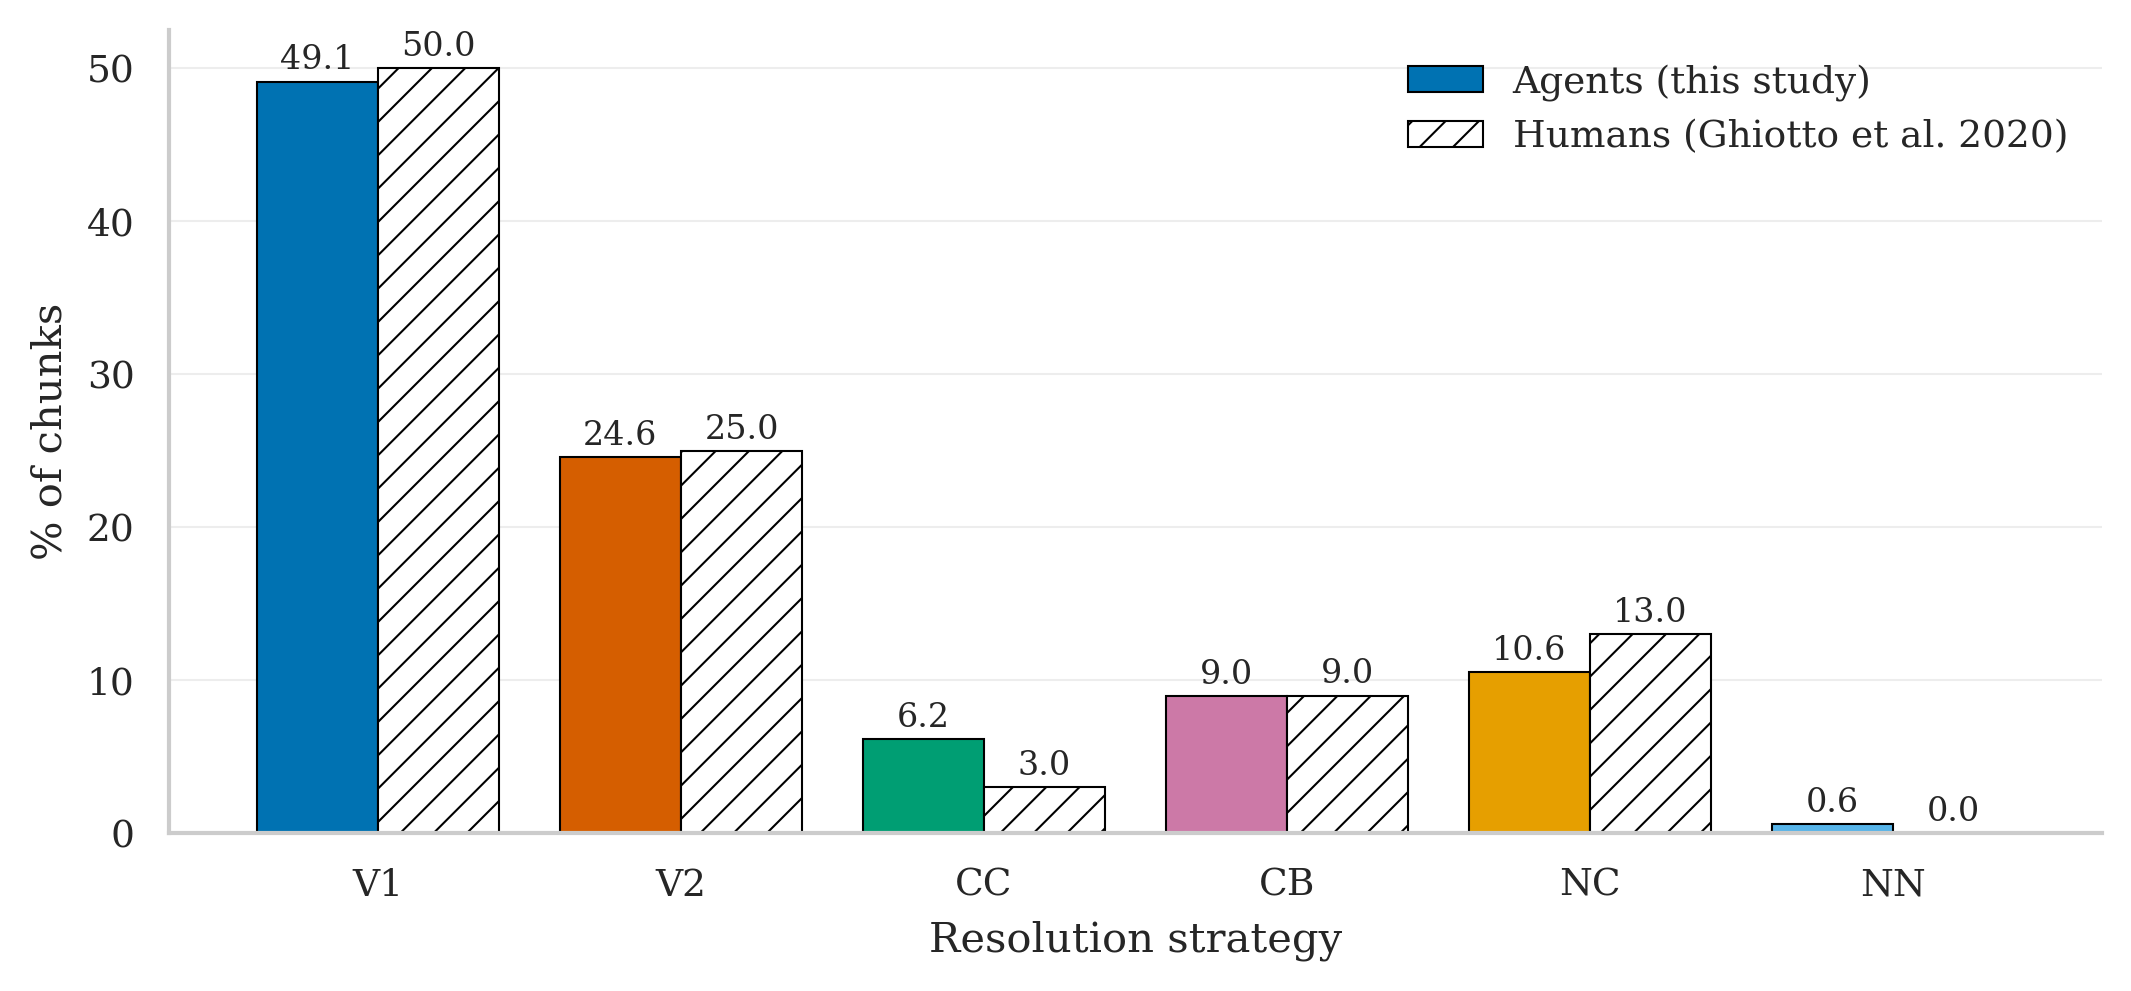
\includegraphics[width=\columnwidth]{rq2_global_vs_ghiotto_excl_imprecise}
  \caption{Global resolution strategy distribution for agent-authored merges (this study, $n{=}60{,}813$ classifiable chunks) versus the human Java baseline of \citet{ghiotto2020nature}. Imprecise chunks ($38.2\%$) are excluded; per-stratum rates are reported in the text.}
  \Description{Grouped bar chart comparing V1, V2, CC, CB, NC, NN proportions between this study and Ghiotto et al. The profiles are broadly similar.}
  \label{fig:rq2-global-ghiotto}
\end{figure}

\begin{figure}[t]
  \centering
  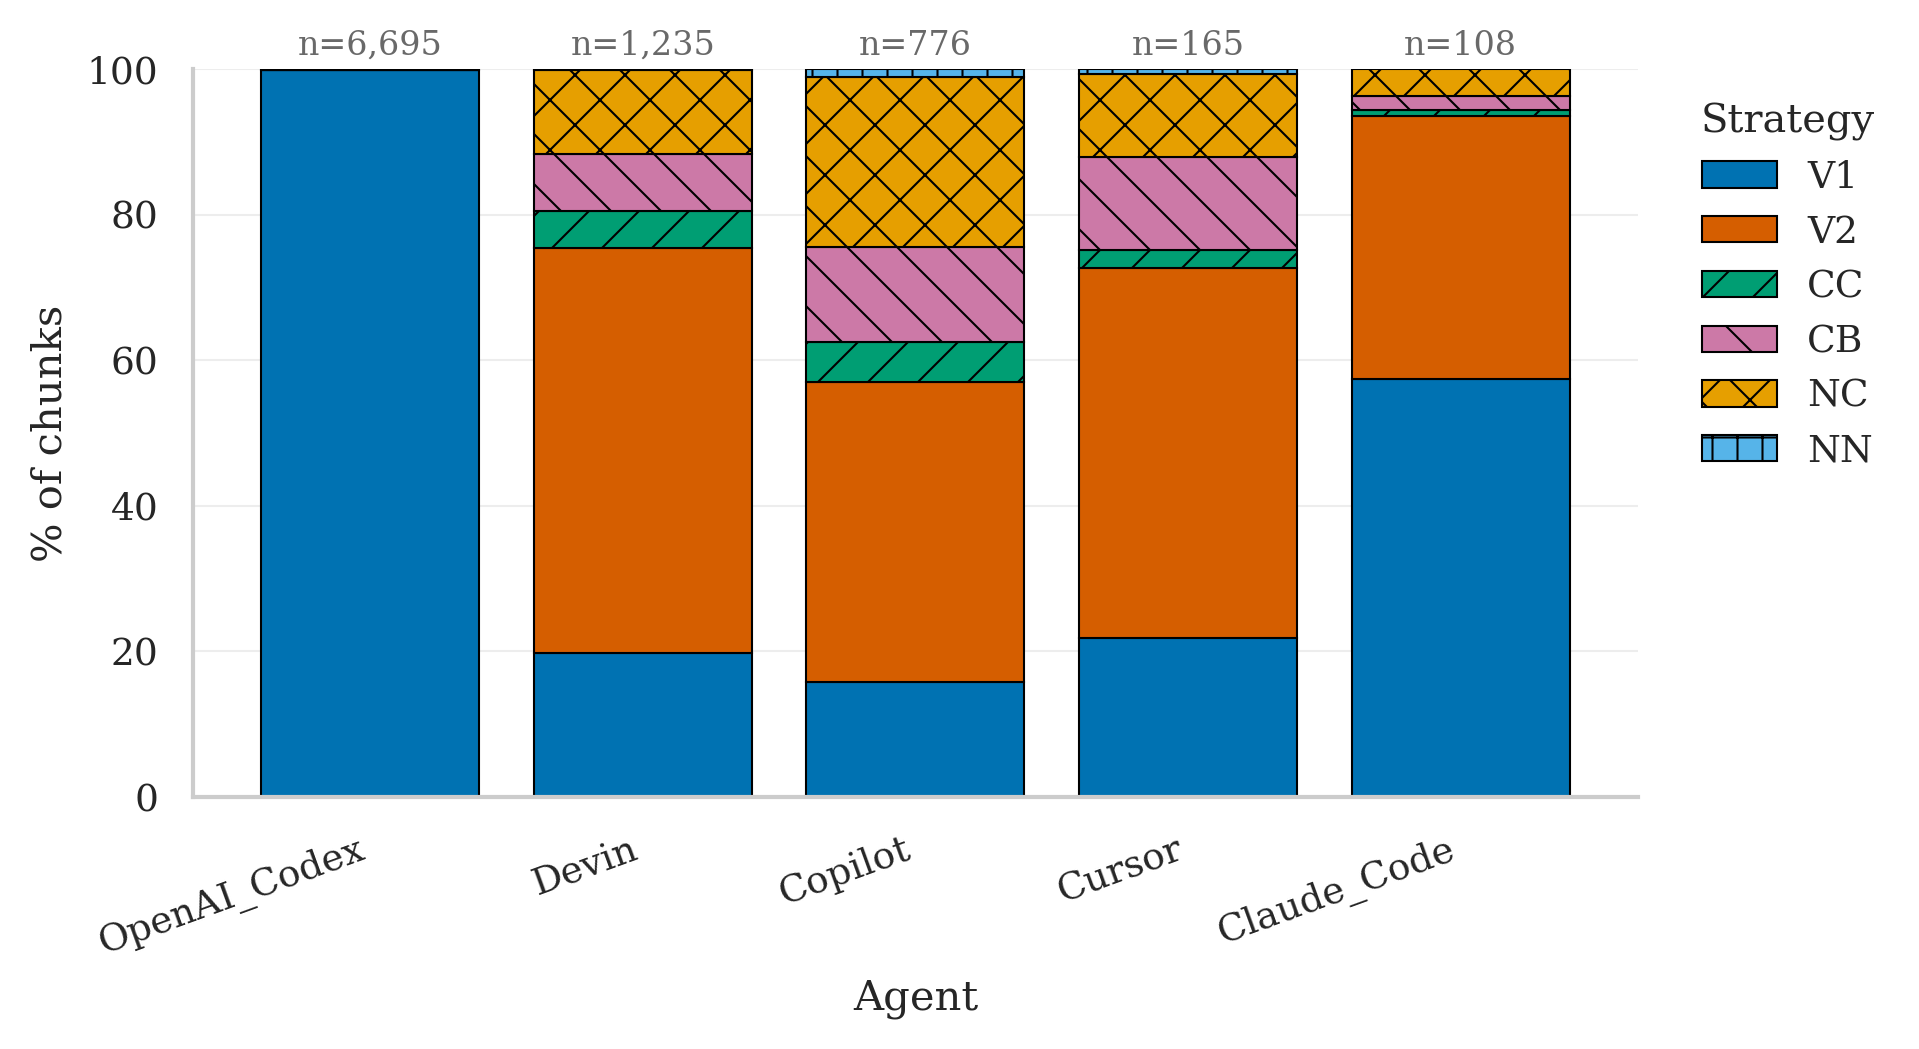
\includegraphics[width=\columnwidth]{rq2_by_agent_excl_imprecise}
  \caption{Resolution strategy distribution per coding agent (Imprecise excluded). The $V_1 / V_2$ polarity inverts for Claude Code and Devin relative to Copilot and OpenAI Codex.}
  \Description{Stacked bar chart showing per-agent strategy breakdown, highlighting the V1/V2 inversion for Claude Code and Devin.}
  \label{fig:rq2-by-agent}
\end{figure}

\begin{figure}[t]
  \centering
  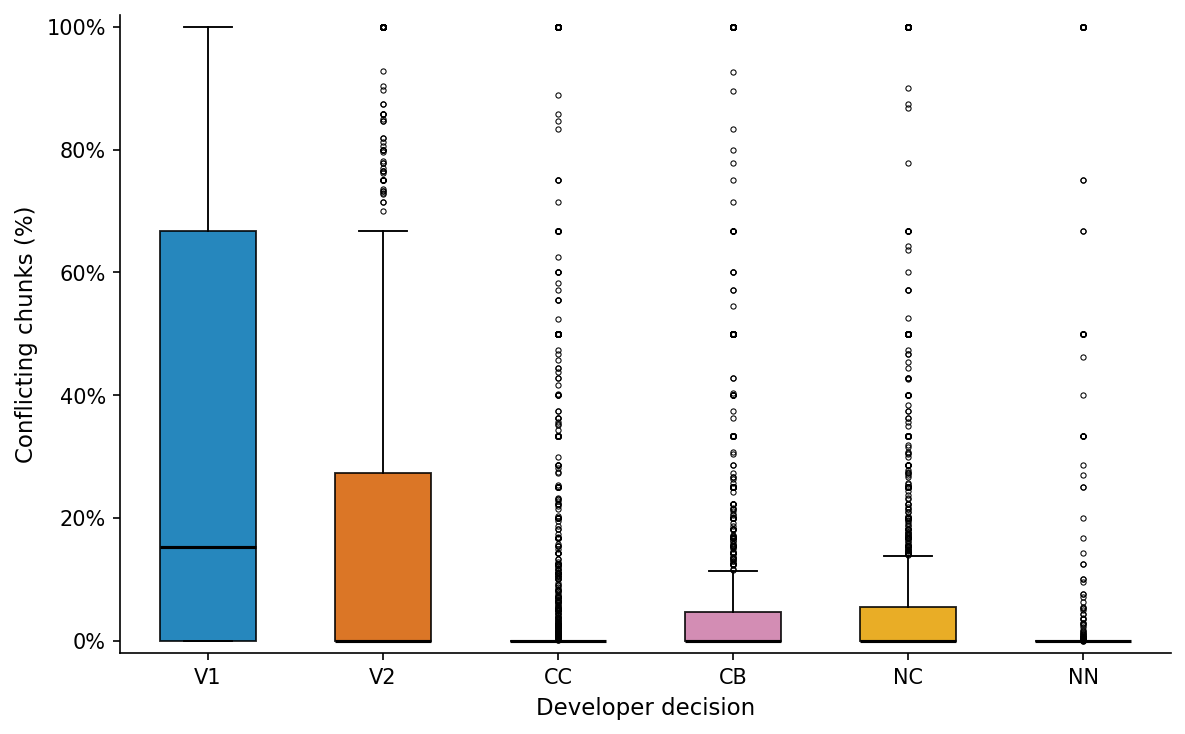
\includegraphics[width=\columnwidth]{rq2_boxplot_by_project}
  \caption{Per-project distribution of the fraction of chunks resolved by each strategy (box plots over all repositories with at least one classifiable chunk). The layout mirrors Fig.~16 of \citet{ghiotto2020nature}, enabling direct visual comparison at the project level.}
  \Description{Box-and-whisker plots for each of the seven strategies showing the distribution of per-project percentages.}
  \label{fig:rq2-boxplot-project}
\end{figure}

\textbf{Summary.} Agent-authored merge conflicts are resolved similarly to human merge conflicts (Figure~\ref{fig:rq2-global-ghiotto}): classifiable resolutions are dominated by verbatim side selection ($74.4\%$ vs.\ $75\%$ for humans), agents write new code slightly less often ($10.4\%$ vs.\ $13\%$), and the mixing rate is slightly higher ($14.6\%$ vs.\ $12\%$). The $V_1$ bias is nearly universal across agents (Figure~\ref{fig:rq2-by-agent}), with two notable inversions (Claude Code and Devin favour $V_2$) and the resolution playbook is broadly comparable to the human baseline. The most striking contrasts emerge when conditioning on the resolver identity, as discussed in Section~\ref{sec:rq3}.

\begin{findingbox}
\textbf{Finding 3.} Among classifiable resolutions, $74.4\%$ adopt one side verbatim (V1~$50.5\%$, V2~$23.9\%$), essentially identical to the $75\%$ reported by Ghiotto~et~al.\ for human Java merges. Agents introduce new code slightly less often ($10.4\%$ vs.\ $13\%$) and mix sides slightly more ($14.6\%$ vs.\ $12\%$). The conservative resolution playbook is a shared trait of the entire agent population (Figure~\ref{fig:rq2-boxplot-project}). \\[3pt]
\textbf{Finding 4.} Two agents (Claude Code, Devin) systematically favour V2 over V1, inverting the global pattern. The NC rate is stable across all agents ($10\%$--$15\%$), confirming that reduced new-code usage is characteristic of the agentic population as a whole, not an artefact of the dominant Codex volume.
\end{findingbox}

\subsection{RQ3: Resolver}
\label{sec:rq3}

\paragraph{Overall resolver distribution.} Across the $40{,}017$ physical internal merges in our dataset, $37{,}658$ ($94.1\%$) are committed by a \emph{human}, $2{,}305$ ($5.8\%$) are committed by the \emph{agent} itself, and $54$ ($0.13\%$) are \emph{agent-assisted}, i.e., merge commits in which an agent-authored trailer (e.g., \texttt{Co-authored-by: devin-ai-integration[bot]}) appears alongside a human committer. The picture is therefore strongly \emph{human-led at the integration step}: even though agents open the PR and produce the feature branch, humans perform the merge in almost fifteen out of sixteen cases.

\paragraph{Per-agent contingency.} Table~\ref{tab:resolver-by-agent} cross-tabulates the PR author against the resolver of the internal merge. The agent-performed share differs by more than an order of magnitude across agents. Devin resolves its own merges most frequently ($19.3\%$, $296$ of $1{,}533$), followed by Claude Code ($9.3\%$, $43$ of $463$), OpenAI Codex ($8.2\%$, $1{,}827$ of $22{,}410$), and Cursor ($7.4\%$, $50$ of $674$); Copilot almost never resolves its own merges ($0.6\%$, $89$ of $14{,}937$). The \emph{agent-assisted} bucket is non-negligible only for Claude Code, where $6.3\%$ of merges carry a human committer plus an agent trailer, suggesting that Claude Code is more often used in an explicitly collaborative ``pair-programming'' mode than the other agents. In absolute terms, OpenAI Codex contributes most of the agent-resolved volume ($1{,}827$ merges, $79\%$ of all agent resolutions in the dataset), simply because it dominates the PR population.

\begin{table}
  \caption{Resolver of the internal merge by PR-authoring agent (merge-commit level).}
  \label{tab:resolver-by-agent}
  \begin{tabular}{lrrrr}
    \toprule
    Agent & Agent & Assisted & Human & Agent~\% \\
    \midrule
    OpenAI Codex & $1{,}827$ & $16$ & $20{,}567$ & $8.2\%$ \\
    Copilot      & $89$      & $4$  & $14{,}844$ & $0.6\%$ \\
    Devin        & $296$     & $2$  & $1{,}235$  & $19.3\%$ \\
    Cursor       & $50$      & $3$  & $621$      & $7.4\%$ \\
    Claude Code  & $43$      & $29$ & $391$      & $9.3\%$ \\
    \midrule
    Total        & $2{,}305$ & $54$ & $37{,}658$ & $5.8\%$ \\
    \bottomrule
  \end{tabular}
\end{table}

\paragraph{Statistical tests.} A chi-squared test of independence between the resolver type (agent / human / agent-assisted) and the coding agent at the merge level yields $\chi^2(8){=}2821$, $p{<}0.001$, Cram\'{e}r's~$V{=}0.19$ (moderate effect), confirming that resolver propensity is not uniform across agents. Per-agent Wilson CIs on the self-resolution rate clearly separate Devin ($19.3\%$, 95\%~CI $[17.4\%,21.4\%]$) from Codex ($8.2\%$, $[7.8\%,8.5\%]$) and Copilot ($0.6\%$, $[0.5\%,0.7\%]$); Claude Code ($9.3\%$, $[7.0\%,12.3\%]$) and Cursor ($7.4\%$, $[5.7\%,9.6\%]$) occupy intermediate positions. The agent-assisted bucket is non-negligible only for Claude Code ($6.3\%$, $[4.4\%,8.9\%]$); for all other agents the assisted CI is below $1.3\%$.

\paragraph{Resolver $\times$ strategy.} The resolver attribution recovers the single largest effect in our data (Figure~\ref{fig:rq3-resolver-strategy}). The \emph{Imprecise} share alone differs markedly: $13.4\%$ of chunks in agent-resolved merges fail to localize, versus $40.8\%$ of chunks in human-resolved merges, consistent with agents producing tighter, more clearly anchored resolutions. Conditioning on classifiable chunks, agent resolvers concentrate $86.6\%$ (95\%~CI $[85.9\%,87.3\%]$) of their decisions on $V_1$ and only $3.2\%$ on new code, whereas human resolvers spread their decisions across all strategies ($V_1$ $45.1\%$, $[44.7\%,45.6\%]$; $V_2$ $26.3\%$; $NC$ $11.5\%$; $CB$ $10.1\%$; $CC$ $6.3\%$). A chi-squared test of independence between strategy and resolver yields $\chi^2(5){=}4819$, $p{<}0.001$, Cram\'{e}r's~$V{=}0.28$ (moderate, approaching strong); this is the largest effect observed in the study. A sensitivity analysis treating all Imprecise chunks as V1 (upper bound) or as NC (lower bound) shows that the agent-to-human V1 ratio remains at $1.31{\times}$--$2.81{\times}$ across all scenarios, confirming that the finding is robust to the differential Imprecise rate. The $54$-merge agent-assisted sample is too small to support strong claims, but its distribution sits between the two regimes, favouring $V_2$ ($50.1\%$) over $V_1$ ($19.5\%$).

\begin{figure}[t]
  \centering
  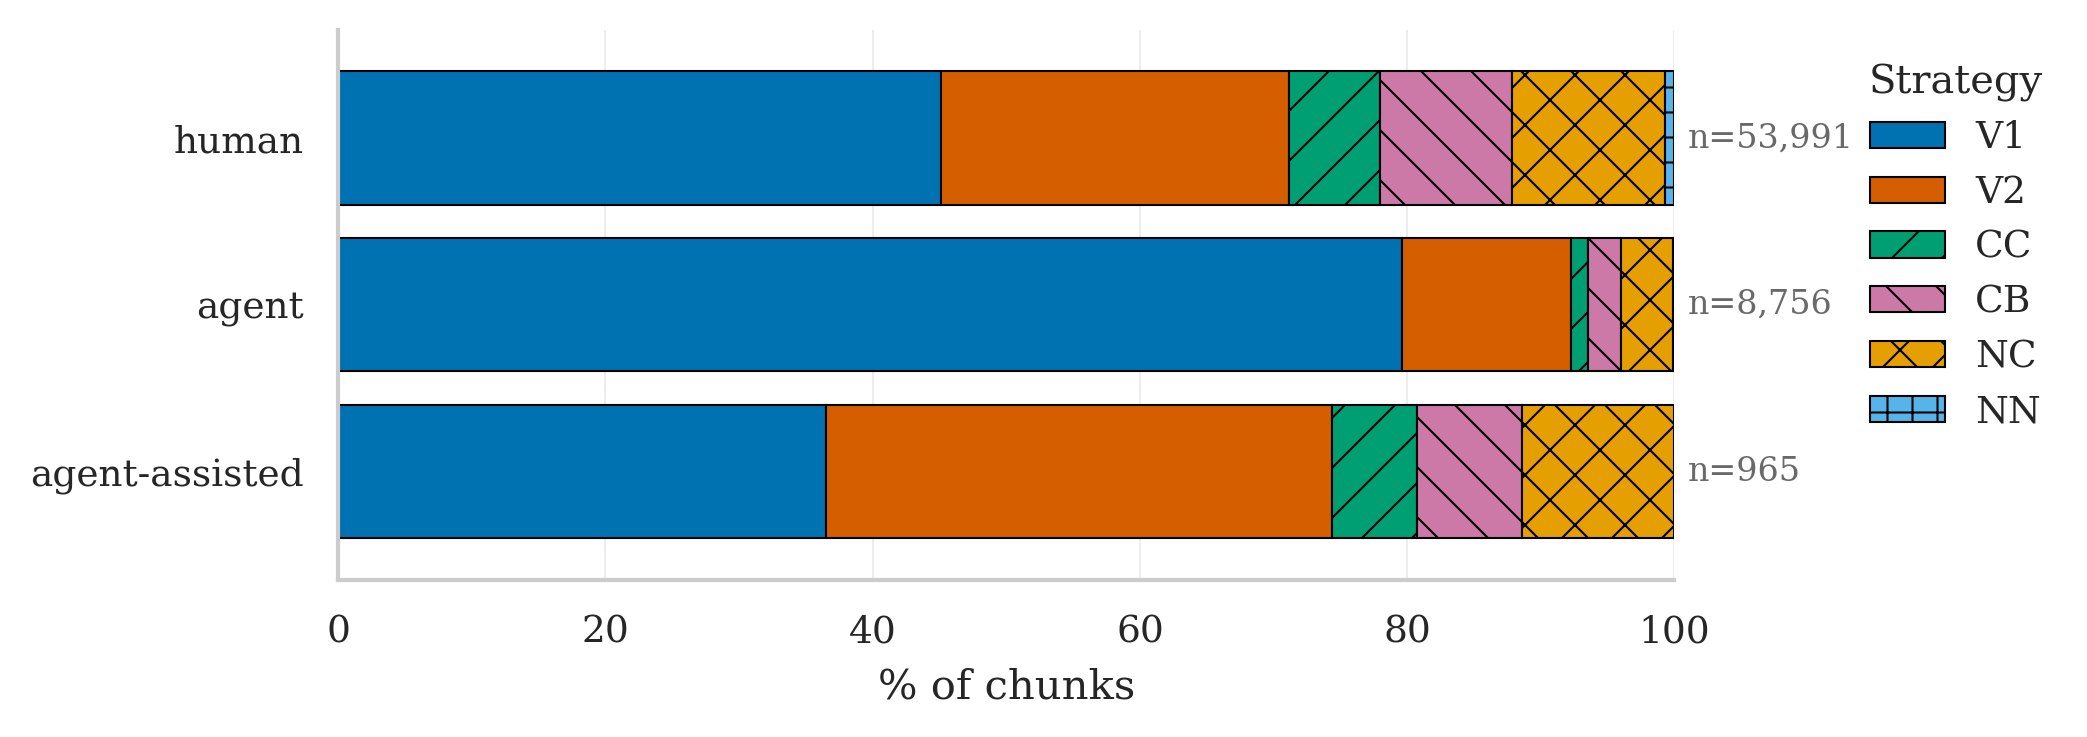
\includegraphics[width=\columnwidth]{rq2_fig16_by_resolver_excl_imprecise}
  \caption{Resolution strategy distribution conditioned on the resolver (agent vs.\ human), Imprecise excluded. This is the largest effect observed in the study: agent resolvers concentrate $86.6\%$ of decisions on $V_1$, while human resolvers spread decisions across all strategies.}
  \Description{Side-by-side bar chart comparing strategy profiles for agent-resolved versus human-resolved chunks, showing the stark V1 dominance for agents.}
  \label{fig:rq3-resolver-strategy}
\end{figure}

\textbf{Summary.} RQ3 shows that integration of agent-authored branches is still \emph{predominantly human-driven} ($94.1\%$ of internal merges are human-committed) and that the propensity of an agent to close its own merges varies by an order of magnitude across vendors, from essentially never (Copilot, $0.6\%$) to roughly one merge in five (Devin, $19.3\%$). When agents do resolve, their strategy profile is strikingly different from both the PR-wide distribution and from the human baseline: $86.6\%$ $V_1$ selection, a near-absence of new-code resolutions, and a three-times-lower Imprecise rate than humans.

\begin{findingbox}
\textbf{Finding 5.} Integration of agent-authored branches is overwhelmingly human-led: $94.1\%$ of internal merges are committed by a human. The agent self-resolution rate varies by more than $30\times$ across vendors, from Copilot ($0.6\%$) to Devin ($19.3\%$). \\[3pt]
\textbf{Finding 6.} When agents resolve their own merges, they select $V_1$ in $86.6\%$ of classifiable chunks, nearly double the human rate of $45.2\%$, and produce almost no new-code resolutions ($3.2\%$ vs.\ $11.5\%$). This is the largest single effect in the study (Cram\'{e}r's~$V{=}0.28$), and it suggests that agents fall back to the simplest possible resolution strategy when acting autonomously (Figure~\ref{fig:rq3-resolver-strategy}).
\end{findingbox}

% ============================================================
% 5. Discussion
% ============================================================
\section{Discussion}
\label{sec:discussion}

\subsection{Key Findings and Implications}
\label{sec:disc-findings}

Our results reveal a coherent picture of \emph{conservative, human-delegated} merge conflict resolution in agent-authored branches. Three themes stand out.

\paragraph{Agents rely on verbatim strategies.} The global rate of verbatim side selection ($74.4\%$) matches the human Java baseline almost exactly, but the within-verbatim structure differs: agents disproportionately favour the \emph{first parent} ($V_1$, $50.5\%$ vs.\ $V_2$, $23.9\%$). This asymmetry likely reflects the typical branch topology: the first parent ($p_1$) is the feature-branch tip authored by the agent, so taking $V_1$ amounts to keeping the agent's own code over the upstream changes. The exceptions (Claude Code and Devin systematically favour $V_2$) hint at agent-specific integration conventions: both tools may be configured to prefer pulling in the upstream state when conflicts arise. The reduced NC rate ($10.4\%$ vs.\ $13\%$) suggests that agents rarely synthesize a wholly new resolution when the two sides conflict, preferring instead to commit deterministically to one side. This conservatism makes agent resolutions more predictable but potentially less semantically correct than human resolutions that write new code.

\paragraph{Conflict incidence is agent- and language-specific.} The six-fold variation in merge-level conflict rates (Copilot $7.8\%$ to Cursor $46.1\%$) cannot be explained by code quality alone; it more likely reflects differences in branching strategy, PR lifetime, and rebasing practice. Copilot tends to produce short-lived, task-focused PRs with infrequent internal merges, while Cursor and Codex branches appear to live longer and incorporate more upstream changes. Language is also a moderating factor: C and TypeScript branches contribute the bulk of the $V_1$ bias, while C\# and C++ show more balanced or $V_2$-dominant profiles. Tooling designers and repository maintainers should therefore calibrate conflict-related settings per agent, not globally.

\paragraph{Human integration dominates.} The $94.1\%$ human resolver share indicates that, in the current ecosystem, agents open branches but rarely close their own merges. This division of labour exposes a gap in the agentic workflow: agents produce and propose changes, but the critical integration step (resolving conflicting regions and verifying semantic correctness) almost always falls to a human. The agent-resolved cases ($5.8\%$) are instructive precisely because they show what agents do when left to their own devices: they pick $V_1$ in $86.6\%$ of chunks, a rate nearly double the human baseline. This strong $V_1$ preference is consistent with a strategy of ``take my own code'' and move on, which minimises the risk of introducing bugs from the upstream version but also ignores the possibility that the upstream edit was intentional and important.

\subsection{Implications for Tool Design}
\label{sec:disc-tools}

Our findings have direct implications for the design of AI-assisted merge tools and CI/CD pipelines involving coding agents.

\paragraph{Targeted resolver augmentation.} Because human resolvers are responsible for $94.1\%$ of all resolutions, and they produce a richer strategy mix (including $11.5\%$ NC and $10.1\%$ CB), merge-assistance tools should be designed primarily for human reviewers, not agents. The human-directed resolution is more semantically nuanced and therefore more error-prone; tools that suggest reference resolutions or flag semantically suspicious verbatim picks would add the most value here. Conversely, agent-performed resolutions are highly predictable ($86.6\%$ $V_1$) and therefore easier to validate automatically: a CI check that flags agent-resolved merges where $V_1$ was not the unique minimum-diff choice would catch the cases most likely to contain silent regressions.

\paragraph{Conflict-complexity triage.} The median conflicting merge contains only two chunks of 2--3 LOC each, placing it well within the range that automated resolvers~\cite{dinella2022deepmerge,svyatkovskiy2022mergebert,dong2023mergegen} handle reliably. However, the heavy right tail (a small fraction of merges above the 99th percentile contains hundreds or thousands of chunks) indicates that a tiered escalation strategy is warranted: resolve the bulk of the conflict load automatically, then route the extreme tail to human reviewers or specialized tooling. The per-agent conflict rates suggest that this triage should be tuned per agent, since Copilot branches are far less likely to produce multi-chunk conflicts than Cursor or Codex branches.

\paragraph{Imprecise rate as a pipeline health signal.} The $38.2\%$ global Imprecise rate, and its $3\times$ variation across resolver types ($13.4\%$ for agent-resolved vs.\ $40.8\%$ for human-resolved), suggests that the Imprecise rate can serve as a \emph{health signal} in merge pipelines. A rising Imprecise rate in a project's history may indicate increasing structural complexity or expanding scope of merge-time edits, either of which warrants attention.

\subsection{Collaborative Dynamics Between AI and Humans}
\label{sec:disc-collaboration}

The clearest take-away about human--AI collaboration from our data is that it is \emph{currently asymmetric}: agents author the branch, but humans integrate it in $94.1\%$ of cases. This mirrors earlier observations about bot-authored PRs~\cite{alfadel2023dependabot}, where human review is the norm even for routine, automated changes. The agent-assisted category ($0.13\%$) is too small to draw strong conclusions, but its elevated $V_2$ rate suggests a collaborative pattern in which the human overrides the agent's edit and defers to the upstream version.

A notable exception is Devin ($19.3\%$ self-resolution rate), which is designed for more extended agentic workflows where the agent is expected to handle not just code generation but also branch maintenance. Claude Code occupies an intermediate position: its $6.3\%$ agent-assisted rate, significantly higher than other agents, suggests it is frequently used in a \emph{pair-programming} mode, where a human co-author watches and guides the agent through the merge. Future work should investigate whether these collaboration patterns correlate with PR acceptance rates and post-merge defect rates.

% ============================================================
% 6. Threats to Validity
% ============================================================
\section{Threats to Validity}
\label{sec:threats}

In this section, we discuss the main threats to the validity of our study, organized according to the categories proposed by \citet{wohlin2012experimentation}: construct validity, internal validity, external validity, and conclusion validity. For each threat, we describe the potential impact and the mitigation actions we adopted.

\subsection{Construct Validity}
\label{sec:threats-construct}

\paragraph{Replay versus historical merge behavior.}
Our pipeline replays the three-way merge between the parents of each internal merge commit using \texttt{git merge-file} with the default \texttt{diff3} algorithm. Some projects configure custom merge drivers (e.g., for generated files, lock files, or language-specific semantic merging), and in those cases our replay may produce conflict markers where the actual project pipeline would not have, or vice versa. The practical impact is that we may over- or underestimate the number of conflicting chunks for individual repositories that rely on non-default merge drivers. This limitation is shared with prior large-scale studies that adopt the same replay methodology~\cite{ghiotto2020nature,boll2024semi,owhadikareshk2019}, and it is an accepted trade-off in exchange for reproducibility and scalability.

\paragraph{Resolution localization.}
The \textsc{LocalizeResRegion} algorithm~\cite{dinella2022deepmerge} identifies the resolution text by anchoring on the prefix and suffix surrounding the conflicting region. When the merge commit introduces edits outside the conflict boundaries (e.g., reformatting, import reordering), the anchoring may fail, and the chunk is classified as \emph{Imprecise}. We mitigate this by reporting the Imprecise rate explicitly in all results and by noting that \citet{dinella2022deepmerge} validated the algorithm on 174 conflict regions with 100\% accuracy (95\% CI: $[0.979, 1.0]$).

\paragraph{Resolution strategy taxonomy.}
Our classification function compares normalized versions of the resolution against $v_1$ and $v_2$ to assign one of seven labels. The normalization strips leading and trailing whitespace and removes blank lines, following \citet{ghiotto2020nature}. Resolutions that differ from a parent version only in whitespace are classified as V1 or V2, which may slightly overcount those strategies. Conversely, minor formatting differences that survive normalization may cause a resolution to be labeled NC. This normalization procedure is the standard adopted in the literature~\cite{ghiotto2020nature,elias2023mestre,camposjunior2022sbes}, making our results directly comparable.

\paragraph{Coverage of ``resolution.''}
Our unit of analysis is the internal merge commit, which does not capture resolutions via interactive rebase (which rewrites history and produces single-parent commits). If a developer resolves a conflict by abandoning the merge and re-implementing changes on a fresh branch, that resolution is invisible to our pipeline. Our study therefore provides a lower-bound characterization of conflict resolution activity in agent-authored PRs, a limitation acknowledged by \citet{ghiotto2020nature} as well.

\subsection{Internal Validity}
\label{sec:threats-internal}

\paragraph{Agent-account mapping.}
We attribute each merge commit to an agent or a human based on the committer identity recorded in the Git metadata. The mapping between account names and agents is derived from the AIDev dataset~\cite{liaidev2026}. Two sources of noise may affect this mapping: agents may have changed their account login over time, and a human developer could theoretically use an agent account (or vice versa). We mitigate this threat by building the definitive account-to-agent mapping from the \texttt{pull\_request.parquet} table grouped by the \texttt{agent} field, which aggregates all known account signatures per agent.

\paragraph{Confounding factors in cross-cutting stratification.}
When stratifying results by coding agent, programming language, or PR task type, confounding factors may influence the observed distributions. Codex dominates AIDev by volume (approximately 76\% of in-scope PRs), so the global distribution is largely driven by Codex's behavior. Similarly, programming language and task type are correlated with the repositories targeted by each agent. We mitigate this by always reporting per-stratum sample sizes alongside the distributions.

\paragraph{Temporal snapshot.}
The AIDev dataset was collected with a cutoff of August 1, 2025~\cite{liaidev2026}. PRs that were still open at that date may have been subsequently merged, closed, or updated. Our analysis treats open PRs as a separate category and does not force an interpretation of abandonment, but the reader should bear in mind the snapshot nature of the data.

\subsection{External Validity}
\label{sec:threats-external}

\paragraph{Public-GitHub scope.}
Our study is scoped to the full AIDev catalogue, restricted to public GitHub repositories. Our findings should not be directly extrapolated to low-visibility or private repositories, which may exhibit different conflict patterns due to differences in project maturity, team size, coding standards, and review practices. Per-task-type analyses rely on the AIDev-pop tier (repositories with more than 100 stars); whenever that stratification is shown, the restricted support is flagged explicitly.

\paragraph{Agent mix.}
The distribution of agents in AIDev is heavily skewed toward Codex (approximately 76\% of in-scope PRs in this study; Table~\ref{tab:scope-per-agent}). Per-agent comparisons involving less represented agents (Claude Code: $463$ internal merges; Cursor: $674$) have wider confidence intervals and lower statistical power. We address this by reporting Wilson CIs for all per-agent proportions, which make the precision of each estimate explicit. Cursor and Claude Code CIs, while wider, remain non-overlapping with the Copilot CI for the key metrics, supporting the qualitative conclusions.

\paragraph{Generalization to future agents.}
The five agents covered in this study represent the most prominent autonomous coding agents available as of mid-2025. The landscape of AI coding agents evolves rapidly, and new agents with different architectures, prompting strategies, or integration workflows may exhibit different conflict resolution behaviors. Our results establish the first empirical baseline for the current generation of agents, but they should be revisited as the ecosystem matures.

\paragraph{Repository and SHA availability.}
Some repositories referenced in the AIDev dataset may have been deleted, made private, or become otherwise inaccessible between the time of data collection and the time of our cloning. Our pipeline covers $57{,}582$ repositories, compared to approximately $116{,}000$ in the full AIDev catalogue; this gap is primarily explained by repositories with no internal merge commits (fast-forward or squash-merge workflows). Only $108$ repositories ($0.2\%$ of in-scope repos) were entirely lost to cloning failures.

Pass B operates on standard bare clones that fetch only permanent branch refs (\texttt{refs/heads/*}). GitHub's PR-specific refs (\texttt{refs/pull/*/head}) are ephemeral infrastructure outside the standard git protocol and are not included in conventional bare clones; this is consistent with how prior large-scale merge mining studies collect data~\cite{ghiotto2020nature,boll2024semi,owhadikareshk2019}. As a consequence, commits that reside solely on a PR branch and have not been incorporated into any permanent branch are not accessible to Pass B. This affects PRs integrated via squash-and-merge or rebase-and-merge (where the original feature-branch commits are discarded in favour of new, rewritten commits on \texttt{main}) and PRs closed without merging. Our Pass B extractor recorded this situation for $247{,}124$ unique SHAs across $88{,}365$ PRs and $15{,}788$ repositories ($27.4\%$ of in-scope repos) as \texttt{sha\_not\_in\_repo}. Our study is therefore scoped to internal merge commits that are part of the repository's permanent git history — precisely those commits that project maintainers chose to preserve. We do not expect this to introduce directional bias with respect to conflict resolution behavior, since the choice of PR integration strategy (squash vs.\ regular merge) is a repository policy largely orthogonal to how conflicts are resolved within the PR.

Finally, $1{,}167$ conflict chunks across $100$ merge commits in $24$ repositories exceeded the per-chunk timeout budget of the \textsc{LocalizeResRegion} algorithm and are classified as \emph{Imprecise}. Since the total Imprecise count is $30{,}791$, timeout-driven failures account for $3.8\%$ of all Imprecise chunks and have negligible influence on the reported strategy distributions.

\subsection{Conclusion Validity}
\label{sec:threats-conclusion}

\paragraph{Statistical test assumptions.}
All chi-squared tests in this study assume independent observations. Conflict chunks within the same merge commit share context (same agent, same codebase, same file), and merge commits within the same repository share project-level factors. This within-cluster correlation means that all reported~$p$-values are anti-conservative. We mitigate this in two ways. First, we report Cram\'{e}r's~$V$ (bias-corrected, Bergsma~\cite{bergsma2013bias}) as the primary effect-size metric rather than relying on $p$-values; $V$ shares the independence assumption but is far less sensitive to~$N$ than~$p$. Second, we treat reported~$V$ values as upper bounds and explicitly flag the clustering caveat in the results. Kruskal-Wallis tests for distributional comparisons (RQ1) are subject to the same within-repo dependence, and Cliff's~$\delta$ is similarly reported as an upper bound.

\paragraph{Power inflation.}
At $n{\approx}60{,}000$ classifiable chunks, the chi-squared tests have extreme statistical power: a difference of $0.1$~pp is sufficient to reach $p{<}0.001$. We therefore do not use statistical significance as evidence of practical importance. Substantive conclusions rest on absolute percentage-point differences and Cram\'{e}r's~$V$; a result is considered practically meaningful only when~$V{>}0.10$ or the absolute difference exceeds several percentage points.

\paragraph{Imprecise differential bias.}
As noted in Section~\ref{sec:meth-resolution}, agent-resolved chunks have a substantially lower Imprecise rate ($13.4\%$) than human-resolved chunks ($40.8\%$). This asymmetry may inflate the apparent~$V_1$ dominance among agent resolvers if $V_1$ resolutions are inherently easier to localize. The sensitivity analysis in Section~\ref{sec:rq3} bounds the agent-to-human V1 ratio at $1.31{\times}$--$2.81{\times}$ across the full range of Imprecise reassignment scenarios, confirming that the qualitative conclusion holds even under the most conservative assumptions.

% ============================================================
% 7. Conclusion
% ============================================================
\section{Conclusion and Future Work}
\label{sec:conclusion}

We presented the first large-scale empirical study of merge conflicts in AI-authored pull requests, covering $40{,}017$ internal merge commits across $57{,}582$ repositories produced by five state-of-the-art coding agents. Our analysis yields three main conclusions.

\textbf{Structural nature (RQ1).} Merge conflicts in agent-authored branches are structurally small, with a median of two chunks of 2--3 LOC, but they exhibit a heavy right tail that concentrates most of the conflict workload in a small fraction of merges. Conflict incidence varies by more than $6{\times}$ across agents (Copilot $7.8\%$ to Cursor $46.1\%$), suggesting that branching strategy and PR lifetime, rather than code quality, are the primary drivers of conflict frequency.

\textbf{Resolution strategies (RQ2).} Among classifiable chunks, $74.4\%$ adopt one side verbatim, essentially matching the $75\%$ reported by \citet{ghiotto2020nature} for human Java merges, while agents introduce new code less often ($10.4\%$ vs.\ $13\%$). The overall distribution is conservative and broadly similar to the human baseline, with the inter-agent variation explained primarily by the $V_1/V_2$ polarity (some agents prefer their own code; others defer to upstream).

\textbf{Resolver (RQ3).} Integration is overwhelmingly human-led: $94.1\%$ of merges are committed by a human. When agents do resolve autonomously, they concentrate $86.6\%$ of decisions on~$V_1$, nearly double the human rate of $45.1\%$, and produce almost no new-code resolutions, an effect confirmed across all sensitivity scenarios (Cram\'{e}r's~$V{=}0.28$).

\paragraph{Future work.} Several directions extend this study naturally. First, a \emph{longitudinal analysis} tracking how conflict rates and resolution strategies evolve as agents mature would establish whether the current baseline is stable or a transient artefact of early adoption. Second, \emph{semantic correctness assessment}, linking each resolution to downstream test outcomes or reviewer comments, would quantify the practical cost of the agent's conservative $V_1$ preference. Third, extending the study to \emph{private repositories} and to newer agent families would test the generalizability of our findings beyond public GitHub. Finally, the patterns documented here can serve as ground-truth labels for training specialized \emph{agentic merge resolution} models, a use case not previously studied.

% ============================================================
% Artifact Availability
% ============================================================
\section*{Artifact Availability}

The dataset and scripts used in this study are publicly available at \emph{[anonymized for review]}. The repository includes all data collection scripts, classification algorithms, statistical analysis notebooks, and figure generation code. The conflict resolution content (v1, v2, base, resolution) is shared as SHA-256 hashes; full text content is available upon request due to licensing considerations.

% ============================================================
% Acknowledgements
% ============================================================
\section*{Acknowledgements}

\emph{[Omitted for double-anonymous review.]} Claude (Anthropic) was used to assist with data analysis scripting and manuscript editing.

% ============================================================
% Bibliography
% ============================================================
\bibliographystyle{ACM-Reference-Format}
\bibliography{references}

\end{document}
